% =====================================================================
% VoiceShield: real-time detection and prevention of voice-cloning
% impersonation in calls (SIH 2026, problem statement SIH26104).
% Single file, no .bib needed. Compile with pdfLaTeX (Overleaf default).
%
% Screenshots (provided next to this file in docs/paper/; upload them to the Overleaf project with these names;
% a grey box "Image file not supplied" is shown until you do):
%   customer.png   /customer page during a HOLD (verdict, signals, bank app)
%   caller.png     /caller page (attacker injecting a recording)
%   security.png   /security dashboard with the incident
%   console.png    command center during a HOLD (provided in docs/paper/)
% Crop browser tabs and the taskbar with the trim values of \shotimg if needed.
%
% BEFORE SUBMISSION: check every number against
% docs/SIH26104_Research_and_Build_Plan.md (Results log) and check the author
% list. References were checked online on 25 Nov 2026 (arXiv, ACL Anthology).
% Step 8b (teacher-anchored consistency LoRA) results of 18 Nov 2026 are
% included: like attempt 1, it did not beat the original model.
% Step 8c (frozen detector + layer back-end + automatic line profile) results
% of 20 Nov 2026 are included, and its integration into the live server with
% the check on real recordings (Step 8d, same day).
% =====================================================================
\documentclass[10pt,a4paper,twocolumn]{article}

\usepackage[margin=18mm,columnsep=8mm,top=22mm,bottom=20mm]{geometry}
\usepackage[T1]{fontenc}
\usepackage[utf8]{inputenc}
\usepackage{mathptmx}
\usepackage{microtype}
\usepackage{graphicx}
\usepackage{adjustbox}
\usepackage{xcolor}
\usepackage{booktabs}
\usepackage{array}
\usepackage{amsmath}
\usepackage{amssymb}
\usepackage{caption}
\usepackage{float}
\usepackage{placeins}
\usepackage{titlesec}
\usepackage{fancyhdr}
\usepackage[authoryear,round]{natbib}
\usepackage{tikz}
\usetikzlibrary{arrows.meta,positioning}
\usepackage{pgfplots}
\pgfplotsset{compat=1.18}
% chart colours (validated categorical slots 1-3; line styles differ too, for print)
\definecolor{seriesA}{HTML}{2A78D6}
\definecolor{seriesB}{HTML}{EB6834}
\definecolor{seriesC}{HTML}{1BAF7A}
\definecolor{gridgrey}{HTML}{E1E0D9}
\definecolor{inkmuted}{HTML}{52514E}
\usepackage[colorlinks=true,linkcolor=black,citecolor=black,urlcolor=black]{hyperref}

% ---------- screenshot helper: crop + scale, or show a placeholder ----
% #1 width, #2 file name, #3 trim = left bottom right top
\newcommand{\shotimg}[3]{%
  \IfFileExists{#2}%
  {\adjustbox{trim={#3},clip,width=#1}{\includegraphics{#2}}}%
  {\fbox{\parbox[c][2.6cm][c]{\dimexpr#1-2\fboxsep-2\fboxrule\relax}{\centering Image file not supplied}}}}

% ---------- caption style: "FIGURE 1 | text" -------------------------
\DeclareCaptionLabelSeparator{bar}{ $\vert$ }
\captionsetup{labelsep=bar,labelfont=bf,font=small,justification=justified,singlelinecheck=false}
\renewcommand{\figurename}{FIGURE}
\renewcommand{\tablename}{TABLE}

% ---------- headings ---------------------------------------------------
\titleformat{\section}{\large\bfseries\sffamily\color{black}}{}{0em}{\MakeUppercase}
\titleformat{\subsection}{\normalsize\bfseries\sffamily}{}{0em}{}
\titlespacing*{\section}{0pt}{10pt}{4pt}
\titlespacing*{\subsection}{0pt}{7pt}{3pt}
\setlength{\parindent}{1.2em}
\setlength{\parskip}{0pt}
\renewcommand{\arraystretch}{1.12}

% ---------- running header / footer -----------------------------------
\pagestyle{fancy}
\fancyhf{}
\fancyhead[R]{\small Real-Time Voice-Clone Impersonation Detection}
\fancyfoot[L]{\small VoiceShield}
\fancyfoot[R]{\small \thepage}
\renewcommand{\headrulewidth}{0.4pt}

\newcommand{\llr}{\ell}

\begin{document}

% =====================================================================
%  TITLE BLOCK + ABSTRACT
% =====================================================================
\twocolumn[
\begin{center}
{\sffamily\bfseries\LARGE VoiceShield: Real-Time Detection and Prevention of Voice-Cloning Impersonation in Calls, and Repairing a Self-Supervised Deepfake Detector Broken by Consumer Audio Processing Without Fine-Tuning\par}
\vspace{8pt}
% CHECK the author list for this project
{\large Alapati Abhinav Chowdhary, Abhishek s, pendyala surya venkata sanjay\par}
\vspace{5pt}
{\small School of Computer Science and Engineering, Lovely Professional University, Phagwara, Punjab, India\par}
{\small Correspondence: \href{mailto:abhinavalapati.aac@gmail.com}{abhinavalapati.aac@gmail.com}\par}
\end{center}
\vspace{4pt}
\noindent\rule{\textwidth}{0.4pt}
\vspace{4pt}

\begin{minipage}{\textwidth}
\small
\noindent\textbf{Abstract.} Voice cloning lets a fraudster speak in the voice of a bank officer, a relative or the account holder, and a call gives the victim little time to doubt it.
We present VoiceShield, a working prototype for the Smart India Hackathon 2026 problem SIH26104 that listens to a live call and returns PASS, VERIFY or HOLD every second, and that blocks a pending bank transfer when the call is judged an impersonation.
It fuses three explainable signals: a pre-trained self-supervised deepfake detector (wav2vec~2.0 Large, post-trained on 74k hours) run on 4-second windows, a voiceprint check against an enrolled customer, and multilingual scam-language rules on a Whisper transcript.
Zero-shot, the detector separated same-speaker voice-conversion clones in Hindi and Telugu (EER 0.0--0.1\%; 1.5--5.2\% after a simulated phone line) and reached 4.7\% EER on an In-the-Wild sample, but 8.2\% on unseen premium commercial voices.
Full fine-tuning on 3,760 in-domain clips did not beat the original on unseen development sets and was rejected.
In live tests on a laptop, a premium AI voice played into the microphone was held after 5.3\,s while the same script read by a person passed, and in a two-browser WebRTC call an injected scam recording was held after about 4\,s of speech and the transfer was blocked automatically.
We also found that consumer audio processing is a major hidden failure mode: operating-system microphone enhancements turned a genuine voice into a false alarm, noise suppression raised the EER on premium clones from 8.2\% to 34.0\% and the Opus codec to 45.1\%, and Opus flagged 32.7\% of real voices at the default threshold.
Two parameter-efficient fine-tuning methods (LoRA, 1.1\% of the weights), one with the label loss only and one anchored to the original model by a teacher-student consistency loss, both learned Bluetooth and Opus conditions on development data but lost accuracy on real-world fakes (In-the-Wild development EER 4.0\% to 9.5\%), so the original model was kept.
We then left the detector frozen. Linear probes on its 25 hidden layers showed that the middle transformer blocks keep the most evidence under processing and that much of the damage is in the original read-out, not in the representation. A layer-weighted back-end with 1,050 parameters, fused with the original head, reduced the mean EER over 13 unseen test sets from 9.7\% to 4.1\%: on premium clones from 8.2\% to 3.0\%, under noise suppression from 34.0\% to 12.7\% and under Opus from 45.1\% to 16.7\%, with no loss on In-the-Wild (4.7\%). A processing classifier that selects a per-processing threshold reduced Opus false alarms on genuine speech from 32.7\% to 13.3\% for the original detector and to 2.7\% for the fused score, but moved errors rather than reducing them overall. In the live server, with the default thresholds, the fused score raised two premium clones from VERIFY to HOLD while genuine callers stayed at PASS. Its processing classifier recognised real Windows noise suppression, but that processing still caused a false alarm in one of two sessions. We also tested a clone of the enrolled user's own voice, made from two minutes of speech. It nearly passed the voiceprint check (similarity 0.41 against a cut-off of 0.45), but the detector flagged it in every window. The call was held, and the transfer requested during a live call was blocked.
We report the defects we found, negative results and the limits of a small evaluation with simulated processing.

\medskip
\noindent\textbf{Keywords:} audio deepfake detection, voice cloning, anti-spoofing, self-supervised learning, wav2vec 2.0, layer-wise probing, speaker verification, scam detection, LoRA, robustness, real-time systems
\end{minipage}
\vspace{4pt}

\noindent\rule{\textwidth}{0.4pt}
\vspace{8pt}
]

% =====================================================================
\section{Introduction}
Text-to-speech (TTS) and voice-conversion (VC) systems can now imitate a person's voice from a few seconds of public audio. In India this has been used in ``digital arrest'' calls, fake bank calls that ask for a one-time password (OTP), and calls in the voice of a relative who needs money urgently. The Smart India Hackathon 2026 problem statement SIH26104, set by the AICTE Cyber Security Cell, asks for an AI system that detects voice-cloning impersonation in real time and \emph{prevents} the attack: acoustic analysis for synthesis artefacts, checks against the genuine voice of the claimed person, a configurable risk engine, alerts and pre-transaction prompts, privacy-preserving logging and multilingual support (Smart India Hackathon, 2026).

Detecting synthetic speech is harder than test-set accuracies suggest. Detectors trained on one benchmark often fail on real-world fakes, with equal error rates (EER) of 34\% or more (M\"uller et al., 2022), and they can learn shortcuts such as the length of leading silence (M\"uller et al., 2021). Self-supervised (SSL) speech models such as wav2vec~2.0 (Baevski et al., 2020) generalise much better (Tak et al., 2022a), and post-training on tens of thousands of hours of real and fake speech has produced detectors that work zero-shot on many data sets (Ge et al., 2025). A call adds more difficulty: the audio is short, compressed by codecs and processed by noise suppression and gain control before any detector sees it. Speaker verification alone does not solve the problem either, because a good clone matches the target voice (Jung et al., 2022).

This paper describes VoiceShield and reports what we measured, including negative results. Our contributions are:
\begin{itemize}\setlength\itemsep{0pt}
  \item a streaming system that fuses a synthetic-voice detector, a voiceprint check and scam-language rules into an explainable PASS/VERIFY/HOLD decision that only escalates, with per-line calibration and no stored audio;
  \item a two-party WebRTC call demonstrator with a prevention workflow: an out-of-band OTP or call-back for VERIFY and an automatic payment block for HOLD;
  \item an evaluation of a strong zero-shot detector on Indian-language same-speaker clones, a simulated phone line, modern commercial TTS and In-the-Wild data, and a fine-tuning experiment that was rejected by model selection on unseen development sets;
  \item a measurement of how consumer audio processing (operating-system enhancements, noise suppression, auto-gain, Bluetooth and VoIP codecs) affects the detector, and two LoRA fine-tuning methods against it, including a teacher-anchored consistency loss, both rejected by model selection on unseen development sets;
  \item a repair that leaves the detector frozen: a layer-wise probe analysis that locates where the evidence survives processing, a layer-weighted back-end fused with the original head that more than halves the mean test EER without forgetting, and a processing classifier that selects a per-processing threshold automatically;
  \item a catalogue of the defects found during development and their fixes.
\end{itemize}

% =====================================================================
\section{Related Work}
\textbf{Generalisation of deepfake speech detectors.} The ASVspoof challenges (Wang et al., 2020; Liu et al., 2023; Wang et al., 2024) established the standard benchmarks for spoofed speech. M\"uller et al. (2022) showed that models trained on ASVspoof 2019 reached EERs of 34\% or more on In-the-Wild, a set of real celebrity and politician deepfakes. M\"uller et al. (2021) found that the duration of leading silence alone predicts the label of ASVspoof 2019, and that trimming silence raised the EER of a RawNet2 model from 6.3\% to 20.8\%. Deepfake-Eval-2024 (Chandra et al., 2025) collected deepfakes circulated on social media and found a large drop in the performance of open-source detectors compared with academic benchmarks.

\textbf{Self-supervised front ends.} Tak et al. (2022a) combined wav2vec~2.0 XLS-R (Babu et al., 2022) with the AASIST graph-attention back end (Jung et al., 2022b) and RawBoost augmentation (Tak et al., 2022b). Zhang et al. (2024) aggregated the hidden layers of XLS-R with a sensitive layer selection (SLS) classifier. A learned weighted sum of all layers of a frozen SSL model is the standard way to use such models for downstream tasks (Yang et al., 2021), and layer-wise probing shows that different blocks of wav2vec~2.0 encode different information (Pasad et al., 2021). Kawa et al. (2023) used Whisper features. Ge et al. (2025) post-trained wav2vec~2.0, HuBERT and MMS models on about 56k hours of real and 18k hours of fake speech in more than 100 languages (``AntiDeepfake''); the released wav2vec~2.0 Large model reports 1.91\% EER on In-the-Wild without further training. We use this model as our detector.

\textbf{Channels and real-time communication.} Codecs, noise and reverberation are known to degrade detectors; the RTCFake corpus re-records real and fake speech through real-time communication platforms for this reason (Xue et al., 2026), and the RADAR 2026 challenge tests detectors under codecs, noise and reverberation (Luong et al., 2026). Our consumer-DSP study (Section~\ref{sec:dsp}) is in this line of work but isolates individual effects that a phone, laptop or headset applies \emph{before} the call codec, and measures false alarms on genuine speech at a fixed threshold as well as EER.

\textbf{Speaker verification and spoofing.} The SASV 2022 challenge (Jung et al., 2022a) showed that a strong speaker-verification system such as ECAPA-TDNN (Desplanques et al., 2020) is easily fooled by spoofed speech, while a spoofing countermeasure is useless for identity, and that fusing the two works best. We follow this idea at decision level, and a matching voice never lowers the risk.

\textbf{Prevention.} Watermarking such as AudioSeal (San Roman et al., 2024) proves that audio came from a cooperating generator, and adversarial perturbation such as AntiFake (Yu et al., 2023) makes published voice samples harder to clone. Neither stops an attacker who uses an open-source cloner. Like most practical systems, we focus on workflow-level prevention: out-of-band verification and blocking a transaction.

\textbf{Parameter-efficient fine-tuning and forgetting.} LoRA (Hu et al., 2022) learns a low-rank update of frozen weights. Fine-tuning a large pre-trained model on a small set can erase what it knew (Kirkpatrick et al., 2017); Learning without Forgetting (Li and Hoiem, 2018) and knowledge distillation (Hinton et al., 2015) keep a model close to its earlier outputs. Our second fine-tuning attempt uses this idea (Section~\ref{sec:dsp}); our third approach avoids forgetting altogether by not changing the detector (Section~\ref{sec:backend}).

% =====================================================================
\section{Background}
\subsection{Detector Score}
The detector maps a 4-second waveform $x$ to two logits $(z_{\text{fake}}, z_{\text{real}})$. We use the log-odds score
\begin{equation}
\llr(x)=z_{\text{fake}}-z_{\text{real}},\qquad p_{\text{fake}}=\sigma(\llr)=\frac{1}{1+e^{-\llr}} ,
\label{eq:llr}
\end{equation}
so that a positive $\llr$ means ``more likely fake''. Clean genuine speech typically scores near $\llr=-10$. The decision threshold on $\llr$ must be calibrated: the optimal probability threshold reported for the model ranges from 0.33 to 0.9995 across data sets (Ge et al., 2025), and a fixed 0.5 is wrong almost everywhere.

\subsection{Equal Error Rate}
With $N_r$ genuine and $N_f$ fake clips and a threshold $\theta$ on $\llr$, the false-alarm rate on genuine speech and the miss rate on fakes are
\begin{equation}
\mathrm{FAR}(\theta)=\frac{|\{i\in\mathcal{R}:\llr_i\geq\theta\}|}{N_r},\quad
\mathrm{MR}(\theta)=\frac{|\{j\in\mathcal{F}:\llr_j<\theta\}|}{N_f}.
\label{eq:far}
\end{equation}
The EER is the common value where $\mathrm{FAR}(\theta^{*})=\mathrm{MR}(\theta^{*})$. EER measures how well the scores \emph{rank} the clips. A deployed system works at one threshold chosen in advance, so we also report FAR and MR at a threshold calibrated on development data.

\subsection{Low-Rank Adaptation}
For a frozen weight matrix $W_0\in\mathbb{R}^{d\times k}$, LoRA adds a trainable update of rank $r$,
\begin{equation}
h=W_0x+\frac{\alpha}{r}BAx,\qquad B\in\mathbb{R}^{d\times r},\;A\in\mathbb{R}^{r\times k},
\label{eq:lora}
\end{equation}
with $B$ initialised to zero (Hu et al., 2022). At step~0 the adapted model is therefore identical to the original, which lets us treat the original model as one candidate checkpoint during model selection.

% =====================================================================
\section{Methods}
\subsection{Threat Model and Scope}
The target is a bank customer who receives a call. The attacker (i) plays a TTS or VC clone of a bank officer, a relative or another person into the call, (ii) is a human who claims to be someone the customer knows, or (iii) reads a scam script in their own voice. The attacker can use commercial or open-source cloners and can call over a VoIP application. Stock Android does not let applications read cellular call audio, so, like other SIH26104 prototypes, we demonstrate on a WebRTC call that we control (Section~\ref{sec:call}). The system gives a warning and triggers bank-side workflow; it does not end calls by itself.

\subsection{Data}
Every source of genuine speech used for training or evaluation is matched by fake speech from the same speakers or the same kind of channel where possible, because otherwise a model can learn ``which data set is this'' (M\"uller et al., 2021). Table~\ref{tab:data} lists the sources. Splits are by speaker, and the commercial voices used for development (Hume) and testing (ElevenLabs, Kokoro) are never used for training.

\begin{table}[t]
\centering\footnotesize
\caption{\textbf{Data used in this work.} kNN-VC clones were generated by us from each speaker's own reference clips.}
\label{tab:data}
\begin{tabular}{@{}p{0.30\columnwidth}p{0.36\columnwidth}p{0.22\columnwidth}@{}}
\toprule
\textbf{Source} & \textbf{Content} & \textbf{Use}\\
\midrule
Kathbath (Javed et al., 2023) & read Hindi and Telugu speech, genuine & Steps 2--4, 8, 8c\\
kNN-VC clones (Baas et al., 2023) & 20 speakers per language, 25 clones each & Steps 3, 4, 8, 8c\\
IndicSynth (Sharma et al., 2025) & XTTS-v2, VITS, FreeVC clones of Kathbath speakers & Steps 2, 4\\
Commercial TTS set (Stafford, 2025) & Polly, Speechify, Luvvoice (train); Hume (dev); ElevenLabs, Kokoro (test) & Steps 2, 4, 5, 8, 8c\\
In-the-Wild (M\"uller et al., 2022) & real-world celebrity deepfakes, English & dev and test samples\\
Own recordings & a team member's voice on a laptop microphone (with consent), ChatGPT voice played from a speaker, a Windows TTS scam script & live tests, calibration\\
\bottomrule
\end{tabular}
\end{table}

\textbf{Same-speaker clones (Step 3).} For 20 Kathbath speakers in each of Hindi and Telugu (gender-balanced) we took 25 genuine clips and made 25 kNN-VC conversions per speaker from about 40 of that speaker's own reference clips: 500 genuine and 500 fake clips per language, split by speaker into 14 training, 3 development and 3 test speakers. A phone version passes each clip through a 300--3400\,Hz band, 8\,kHz sampling and G.711 $\mu$-law coding (ITU-T, 1988). When listening, we noticed that the clones sounded \emph{cleaner} than the genuine clips, so a model trained on them as they are could learn ``clean means fake''. All later training therefore applies the same random noise and channel effects to both classes.

\subsection{Synthetic-Voice Detector}
We use the AntiDeepfake wav2vec~2.0 Large model (Ge et al., 2025): a convolutional feature encoder, 24 transformer blocks (about 315\,M parameters), mean pooling over time and a two-way linear head. For serving we use an ONNX export and ONNX Runtime on the CPU. The input is 16\,kHz mono audio, normalised to zero mean and unit variance per window; the window is 4.0\,s (64,000 samples). For training we rebuilt the model in PyTorch and checked that it matches the ONNX model (maximum logit difference 0.0001). The model is released under CC BY-NC-SA, which restricts our work to non-commercial use.

\subsection{Fine-Tuning Experiment (Step 4)}
We fine-tuned the full detector on 3,760 clips (1,884 genuine, 1,876 fake): 700 genuine and 700 kNN-VC clips of the Step 3 training speakers, 600 extra Kathbath clips, 600 IndicSynth fakes, and 584 genuine and 576 commercial TTS clips. Augmentation was identical for both classes: noise at 5--30\,dB SNR, denoising, the phone channel and low-pass filtering. We used AdamW with a backbone learning rate of $5\times10^{-6}$, a head learning rate of $5\times10^{-5}$, a batch of 16 and a frozen convolutional front end. Model selection used the mean EER of four development sets: held-out speakers clean, held-out speakers phone, unseen Hume voices and an In-the-Wild development sample. The original model counted as step~0, and training stopped after four evaluations without improvement.

\subsection{Streaming Pipeline}
The server is written in Python with FastAPI. A client sends 16-bit PCM in chunks of about 100\,ms over a WebSocket; other sample rates go through a streaming resampler with an elliptic anti-aliasing filter. Silero VAD v5 (Silero Team, 2024) labels each 32\,ms frame with a 300\,ms hangover, and only speech is kept. Once 2\,s of speech has arrived, a rolling 4\,s window of speech is analysed after every 1\,s of new speech. The detector, the speaker model and the speech recogniser each run in their own thread pool, so a slow transcript never delays the voice decision.

\subsection{Line Profiles}
\label{sec:profiles}
The detector's raw score depends on the channel (Section~\ref{sec:mic}), so every input line has a profile with its own threshold $\theta_{\ell}$ on $\llr$:
\begin{itemize}\setlength\itemsep{0pt}
\item \texttt{default}: $-4.07$, the EER threshold of the pooled Step 4 development sets ($p_{\text{fake}}=0.0168$);
\item \texttt{studio}: $-5.63$, the window-level EER threshold on the development split of the commercial TTS set (116 genuine clips of 4 speakers, 116 Hume fakes; window EER 2.1\%);
\item lines calibrated from genuine speech only, such as the laptop microphone (\texttt{mic}):
\begin{equation}
\theta_{\ell}=\mathrm{clip}\big(Q_{0.95}(\llr_{\text{genuine}})+1.5,\;-9.5,\;0\big),
\label{eq:calib}
\end{equation}
where $Q_{0.95}$ is the 95th percentile of the genuine window scores.
\end{itemize}

\subsection{Voiceprint Check}
A customer can enrol a voiceprint (at least about 7\,s of speech). We use the WeSpeaker ResNet34-LM model trained on VoxCeleb (Wang et al., 2023; Nagrani et al., 2017), exported to ONNX, with an 80-band Kaldi-style filterbank computed in NumPy so that the server does not need PyTorch. During a call the window embeddings are summed into a running voiceprint $\bar e$, and the mismatch with the enrolled voiceprint $e_{\text{enr}}$ of the claimed person is
\begin{equation}
I=\sigma\!\left(\frac{\tau_s-\cos(\bar e,e_{\text{enr}})}{\beta}\right),\quad \tau_s=0.45,\;\beta=0.08 .
\label{eq:spk}
\end{equation}
The threshold 0.45 lies between the within-speaker similarities (0.60--0.87) and between-speaker similarities (0.00--0.25) that we measured on seven two-person interview recordings.

\subsection{Transcript and Scam Language}
Utterances cut by the VAD (at pauses, at most 8\,s) are transcribed by faster-whisper (Radford et al., 2023) with the \emph{small} model on the laptop GPU and the \emph{base} model as a CPU fallback. Phrases that Whisper is known to hallucinate on silence are removed. The transcript is matched against explainable rules for nine scam tactics (Table~\ref{tab:tactics} in Appendix~A) in English, romanised Hindi and Telugu, Devanagari and Telugu script. Each tactic $k$ has a weight $w_k$, and the tactics $\mathcal{T}$ seen so far in the call combine by noisy-OR,
\begin{equation}
C=1-\prod_{k\in\mathcal{T}}(1-w_k).
\label{eq:scam}
\end{equation}
One neutral mention stays low (``transfer'' alone gives 40 on a 0--100 scale), whereas a bank claim, an account threat, an OTP request and a request for secrecy together give 84.

\subsection{Risk Engine}
For each detector window $t$ the score is turned into a window score and a running synthetic-voice risk,
\begin{equation}
s_t=\sigma\big(\llr_t-\theta_{\ell}\big),\qquad V_t=(1-\alpha)V_{t-1}+\alpha s_t,\quad V_0=0,
\label{eq:ema}
\end{equation}
with $\alpha=0.4$. Starting from $V_0=0$ (genuine) means that one odd first window cannot raise an alert. Let $k_t$ be the number of the last five windows with $s\geq0.5$, and let $V$, $I$ and $C$ be expressed on a 0--100 scale. The decision rules are applied in this order (Figure~\ref{fig:risk}):
\begin{itemize}\setlength\itemsep{0pt}
\item \textbf{HOLD} if $V\geq75$ and $k_t\geq3$ (strong synthetic voice);
\item \textbf{HOLD} if $C\geq50$ and the voice or the identity was suspicious at any time in the call (fused evidence);
\item \textbf{VERIFY} if $V\geq45$, $k_t\geq2$, $I\geq50$ or $C\geq50$;
\item \textbf{PASS} otherwise.
\end{itemize}
The call verdict only escalates. Scam words from a genuine, matching voice therefore give VERIFY, never HOLD, and a matching voice never lowers the risk. For display we combine the signals into one number, $R=1-(1-V)(1-I)(1-C)$, and every alert lists its reasons in plain words, for example ``voice does not match the claimed person (100/100)''.

\begin{figure}[t]
\centering
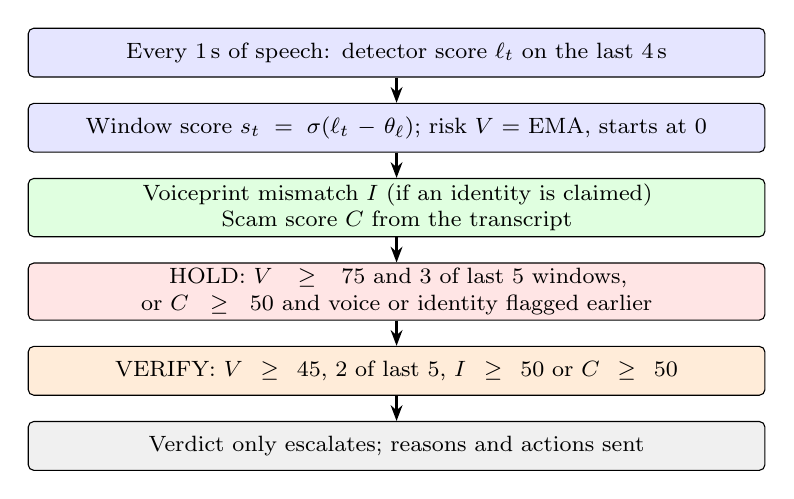
\begin{tikzpicture}[
  node distance=3.2mm,
  box/.style={draw,rounded corners=2pt,align=center,font=\footnotesize,text width=0.76\columnwidth,minimum height=6.2mm,inner sep=2pt},
  arr/.style={-{Stealth[length=2mm]},thick}]
\node[box,fill=blue!10] (a) {Every 1\,s of speech: detector score $\llr_t$ on the last 4\,s};
\node[box,fill=blue!10,below=of a] (b) {Window score $s_t=\sigma(\llr_t-\theta_{\ell})$; risk $V$ = EMA, starts at 0};
\node[box,fill=green!12,below=of b] (c) {Voiceprint mismatch $I$ (if an identity is claimed)\\Scam score $C$ from the transcript};
\node[box,fill=red!10,below=of c] (d) {HOLD: $V\geq75$ and 3 of last 5 windows,\\or $C\geq50$ and voice or identity flagged earlier};
\node[box,fill=orange!15,below=of d] (e) {VERIFY: $V\geq45$, 2 of last 5, $I\geq50$ or $C\geq50$};
\node[box,fill=gray!12,below=of e] (f) {Verdict only escalates; reasons and actions sent};
\foreach \x/\y in {a/b,b/c,c/d,d/e,e/f} \draw[arr] (\x) -- (\y);
\end{tikzpicture}
\caption{\textbf{Risk engine.} Three independent signals, explainable rules and a verdict that never de-escalates during a call.}
\label{fig:risk}
\end{figure}

\subsection{Call Demonstrator and Prevention}
\label{sec:call}
The demonstrator has three web pages (Figure~\ref{fig:overview}). The \texttt{/caller} page is the genuine caller or the attacker; it sends the raw microphone, or \emph{injects a recording into the call} through Web Audio, and can send a payment request. The \texttt{/customer} page answers the call, plays the caller, and streams the \emph{remote} audio to the server; it shows the verdict, the three signals, a risk chart, the transcript and a mock banking app. The security team's \emph{Incidents} view lists the protected calls with their reasons, scam tactics and prevention actions. The browsers are connected by a WebRTC peer connection (W3C, 2021); the server only relays signalling messages. The Opus codec (Valin et al., 2012) is set to mono, 128\,kbit/s and no discontinuous transmission, so that the call codec adds as few artefacts as possible.

The prevention workflow is: PASS allows a payment; VERIFY requires an out-of-band check, either an OTP sent to the customer's registered phone with a ``never share this on a call'' warning, or hanging up and calling back the official number; HOLD blocks a pending or new payment automatically and alerts the security team. Each step is recorded against the call (for example \texttt{TRANSFER\_BLOCKED}, \texttt{OTP\_SENT}, \texttt{CALLBACK\_REQUESTED}). The audit database stores scores, decisions and the \emph{names} of scam tactics only; audio, transcripts and voiceprints are never logged, and voiceprints can be deleted from the console. A single-page console serves the operator and the security team with seven views:
\begin{itemize}\setlength\itemsep{0pt}
\item a live command center;
\item a forensic voice analysis, with waveform, spectrogram and per-window verdicts;
\item the incident list;
\item the detection history;
\item an investigation view that keeps the model's prediction, the supporting signals and the actions taken apart;
\item analytics computed from the audit log;
\item settings for enrolment and calibration.
\end{itemize}
The live waveform is drawn from the same PCM chunks that are streamed to the detector, so it shows exactly the audio being judged, coloured by the verdict at the time it was captured. Status is never shown by colour alone. The pages use no external fonts or libraries, so the demonstration works offline (Figure~\ref{fig:ui}).

\begin{figure*}[t]
\centering
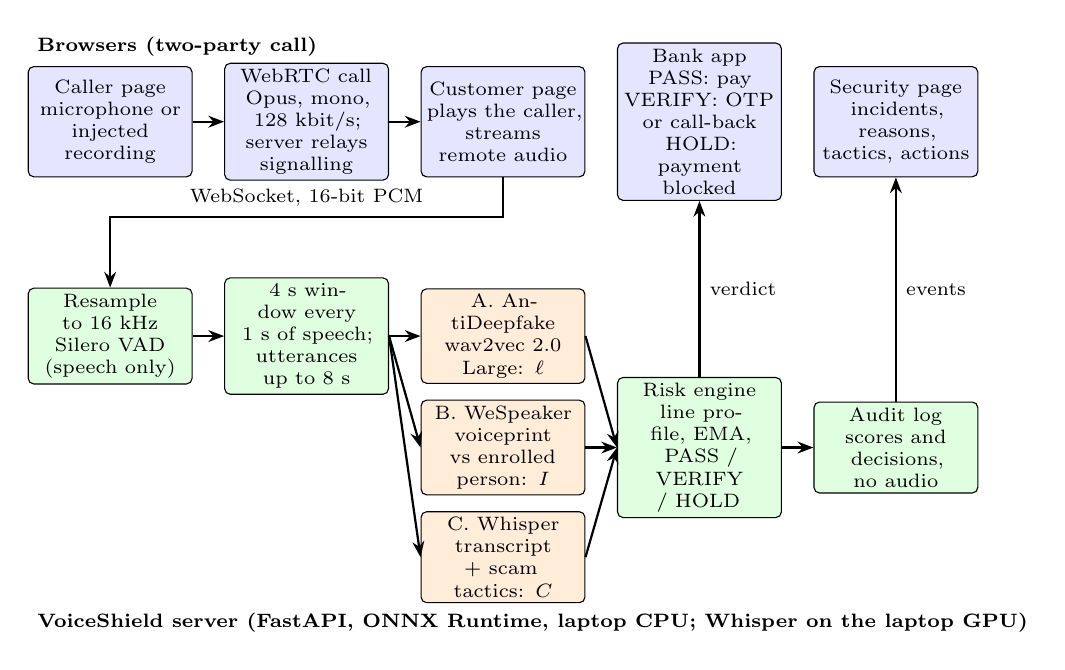
\begin{tikzpicture}[
  box/.style={draw,rounded corners=2pt,align=center,font=\scriptsize,text width=0.16\textwidth,minimum height=11mm,inner sep=2pt},
  web/.style={box,fill=blue!10,minimum height=14mm},
  srv/.style={box,fill=green!12},
  sig/.style={box,fill=orange!15,minimum height=9mm},
  arr/.style={-{Stealth[length=2mm]},thick}]
\node[web] (a1) {Caller page\\microphone or\\injected recording};
\node[web,right=4mm of a1] (a2) {WebRTC call\\Opus, mono, 128 kbit/s;\\server relays signalling};
\node[web,right=4mm of a2] (a3) {Customer page\\plays the caller,\\streams remote audio};
\node[web,right=4mm of a3] (a4) {Bank app\\PASS: pay\\VERIFY: OTP or call-back\\HOLD: payment blocked};
\node[web,right=4mm of a4] (a5) {Security page\\incidents, reasons,\\tactics, actions};
\node[srv,below=14mm of a1] (b1) {Resample to 16 kHz\\Silero VAD\\(speech only)};
\node[srv,right=4mm of b1] (b2) {4 s window every\\1 s of speech;\\utterances up to 8 s};
\node[sig,right=4mm of b2] (b3) {A. AntiDeepfake\\wav2vec 2.0 Large: $\llr$};
\node[sig,below=2mm of b3] (b4) {B. WeSpeaker voiceprint\\vs enrolled person: $I$};
\node[sig,below=2mm of b4] (b5) {C. Whisper transcript\\+ scam tactics: $C$};
\node[srv,right=4mm of b4] (b6) {Risk engine\\line profile, EMA,\\PASS / VERIFY / HOLD};
\node[srv,right=4mm of b6] (b7) {Audit log\\scores and decisions,\\no audio};
\draw[arr] (a1) -- (a2);
\draw[arr] (a2) -- (a3);
\draw[arr] (a3.south) -- ++(0,-5mm) -| node[pos=0.25,above,font=\scriptsize] {WebSocket, 16-bit PCM} (b1.north);
\draw[arr] (b1) -- (b2);
\draw[arr] (b2.east) -- (b3.west);
\draw[arr] (b2.east) -- (b4.west);
\draw[arr] (b2.east) -- (b5.west);
\draw[arr] (b3.east) -- (b6.west);
\draw[arr] (b4.east) -- (b6.west);
\draw[arr] (b5.east) -- (b6.west);
\draw[arr] (b6) -- (b7);
\draw[arr] (b6.north) -- node[right,font=\scriptsize] {verdict} (a4.south);
\draw[arr] (b7.north) -- node[right,font=\scriptsize] {events} (a5.south);
\node[anchor=south west,font=\scriptsize\bfseries] at (a1.north west) {Browsers (two-party call)};
\node[anchor=north west,font=\scriptsize\bfseries] at (b5.south west -| b1.west) {VoiceShield server (FastAPI, ONNX Runtime, laptop CPU; Whisper on the laptop GPU)};
\end{tikzpicture}
\caption{\textbf{System overview.} Blue: browser pages of the call demonstrator. Green: server stages. Orange: the three independent signals. The customer's page streams the audio it \emph{receives} from the caller, so the system hears what the victim hears.}
\label{fig:overview}
\end{figure*}

\begin{figure*}[t]
\centering
\begin{minipage}[t]{0.485\textwidth}\centering
\shotimg{\linewidth}{customer.png}{0pt 0pt 0pt 0pt}\\[2pt]
{\scriptsize (a) Customer page during a HOLD, with the blocked transfer}
\end{minipage}\hfill
\begin{minipage}[t]{0.485\textwidth}\centering
\shotimg{\linewidth}{caller.png}{0pt 0pt 0pt 0pt}\\[2pt]
{\scriptsize (b) Caller page: the attacker injects a recording}
\end{minipage}

\vspace{6pt}
\begin{minipage}[t]{0.485\textwidth}\centering
\shotimg{\linewidth}{security.png}{0pt 0pt 0pt 0pt}\\[2pt]
{\scriptsize (c) Incidents view for the security team}
\end{minipage}\hfill
\begin{minipage}[t]{0.485\textwidth}\centering
\shotimg{\linewidth}{console.png}{0pt 0pt 0pt 0pt}\\[2pt]
{\scriptsize (d) Command center during the demo scam call (HOLD at 4.4 s)}
\end{minipage}
\caption{\textbf{Screenshots of the prototype}, captured from the running system. (a)~The customer sees the verdict, the three signals and the reasons; the banking app blocks the payment. (b)~The caller page can send the microphone or a recording into the WebRTC call. (c)~Incidents with verdict, scam tactics and prevention events. (d)~The command center: verdict and risk, AI-voice probability of the latest window, the three signals, and the system response.}
\label{fig:ui}
\end{figure*}

\subsection{Consumer Audio Processing Study (Step 8)}
\label{sec:dsp}
Live tests showed that processing before the detector can change its scores strongly (Section~\ref{sec:mic}). We therefore implemented seven effects that phones, laptops, headsets and calling apps apply, and measured the detector under each:
\begin{itemize}\setlength\itemsep{0pt}
\item noise suppression by non-stationary spectral gating (Sainburg et al., 2020);
\item spectral subtraction with over-subtraction, a gain floor and temporal smoothing (Boll, 1979);
\item automatic gain control with fast attack, slow release and a soft limiter, alone and followed by spectral subtraction;
\item a G.711 phone line;
\item Bluetooth hands-free CVSD: 8\,kHz with delta modulation at 64\,kbit/s;
\item an mSBC-like wide-band Bluetooth channel: 16\,kHz, 7\,kHz band and 8-bit companding (an approximation, not the real codec);
\item Opus at 8--24\,kbit/s through ffmpeg.
\end{itemize}
In the test sets each effect is applied after background noise at 15\,dB SNR. ``False alarms'' and ``missed fakes'' are measured at the threshold calibrated on the clean development sets, as a deployed system would use it.

\textbf{DSP-aware LoRA, attempt 1.} We froze the detector and trained LoRA adapters (Equation~\ref{eq:lora}; $r=8$, $\alpha=16$, dropout 0.05) on the query, key, value and output projections and both feed-forward layers of all 24 blocks, plus the two-way head: 3.54\,M trainable parameters of 319\,M (1.11\%). The 4,360 training clips received the same augmentation for both classes: noise with probability 0.5, one consumer effect with probability 0.6 and a low-pass filter with probability 0.1. Learning rates were $10^{-4}$ for the adapters and $10^{-5}$ for the head, with an effective batch of 16 in mixed precision. Model selection used the mean EER of eight development sets (held-out speakers clean and phone, Hume, In-the-Wild, noise suppression, auto-gain with spectral subtraction, CVSD and Opus), evaluated every 100 steps; the original model was step~0, and training stopped after four evaluations without improvement. The best adapter would be merged into the backbone and exported to ONNX for the server.

\textbf{DSP-aware LoRA, attempt 2: teacher-anchored consistency.} To counter the forgetting seen in attempt~1, the second attempt keeps the original model as a teacher. For each training clip we take a clean crop $x$ and, in 85\% of cases, a processed copy $\tilde x$ of the \emph{same} crop (noise with probability 0.5, then one consumer effect, or a low-pass filter in 20\% of cases); otherwise $\tilde x=x$. The frozen original model $f_0$ (adapters switched off, frozen copy of the original head) scores $x$, and the adapted model $f_\phi$ is trained on $\tilde x$ with
\begin{equation}
\mathcal{L}=\mathrm{CE}\big(f_\phi(\tilde x),y\big)+\lambda\tau^{2}\,g\,\mathrm{KL}\big(\sigma_\tau(f_0(x))\,\Vert\,\sigma_\tau(f_\phi(\tilde x))\big),
\label{eq:consistency}
\end{equation}
where $\sigma_\tau$ is a softmax at temperature $\tau=2$, $\lambda=1$, and the gate $g\in\{0,1\}$ is 1 only when the original model's decision on the clean crop is correct, so the teacher never teaches a mistake. The model is asked to give the clean-audio answer after processing while staying close to the original model. The adapter learning rate was $5\times10^{-5}$ (head $10^{-5}$) with 100 warm-up steps, and training stopped after six evaluations without improvement; the data, development sets and model selection were the same as in attempt~1.

\subsection{Frozen-Detector Back-End and Automatic Line Profile (Step 8c)}
\label{sec:backend}
Every fine-tuning run changed the detector's weights and lost accuracy on real-world fakes (Section~\ref{sec:dspres}). Step 8c therefore keeps every weight of the detector fixed and trains only small models on its hidden layers. Each 4\,s crop is passed once through the frozen detector, and for each of its 25 hidden layers we keep the mean over the $T$ time frames, standardised with the mean $\mu_l$ and standard deviation $s_l$ of the training views:
\begin{equation}
z_l(x)=\frac{\bar h_l(x)-\mu_l}{s_l},\qquad \bar h_l(x)=\frac{1}{T}\sum_{t=1}^{T}h_{l,t}(x),\qquad l=0,\dots,24 .
\label{eq:layers}
\end{equation}
Layer 0 is the input to the first transformer block and layer 24 is the final output, which the original head reads after the same mean pooling. Because the detector is unchanged, its own score $\llr(x)$ stays available and identical.

\textbf{Training views.} Each of the 4,360 Step~8 training clips gives three views: one clean crop and two processed crops, which receive background noise at 5--30\,dB SNR with probability 0.5 and then, with probability 0.85, one of eight processing types (G.711 phone line, noise suppression, spectral subtraction, auto-gain, auto-gain with spectral subtraction, CVSD, mSBC-like, Opus). Both classes are processed in the same way, and the processing type is kept as a second label. The 13,080 views are encoded once and cached in half precision. The notebook checks that the original head applied to the cached last layer reproduces the detector's score.

\textbf{Layer analysis.} For each layer $l$ we train a logistic-regression probe on $z_l$ (AdamW, learning rate $10^{-2}$, weight decay $10^{-2}$, 300 full-batch steps) and measure its EER on every development and test set. The probes show where the evidence that separates genuine from fake speech survives processing.

\textbf{Back-end and fusion.} Similar in spirit to the weighted layer sum of SUPERB (Yang et al., 2021) and to SLS (Zhang et al., 2024), the back-end learns one weight per layer and a linear read-out,
\begin{equation}
q(x)=\mathbf{v}^{\top}\sum_{l=0}^{24}\pi_l\,z_l(x)+b,\qquad \boldsymbol{\pi}=\mathrm{softmax}(\mathbf{a}),
\label{eq:backend}
\end{equation}
with 1,050 parameters ($\mathbf{a}\in\mathbb{R}^{25}$, $\mathbf{v}\in\mathbb{R}^{1024}$, $b$). It is trained with binary cross-entropy (AdamW, learning rate $10^{-3}$, weight decay $10^{-2}$, batch 256, dropout 0.2 on the pooled vector) for 30 epochs, and the epoch with the lowest mean EER of the eight development sets of Step~8 is kept. The back-end is then fused with the original score,
\begin{equation}
f(x)=(1-w)\,\frac{\llr(x)-m_{\llr}}{s_{\llr}}+w\,\frac{q(x)-m_q}{s_q},
\label{eq:fusion}
\end{equation}
where $m$ and $s$ are the mean and standard deviation over the pooled development sets. The weight $w$ is chosen from $\{0,0.05,\dots,1\}$ by the mean development EER, with ties going to the smaller $w$. At $w=0$, $f$ is a monotone function of $\llr$, so the original detector is always one of the candidates, as in our fine-tuning runs.

\textbf{Automatic line profile.} The line profiles of Section~\ref{sec:profiles} must be chosen by hand. To choose them automatically, a second model with the structure of Equation~\ref{eq:backend} but nine outputs (9,250 parameters) predicts the processing type $\hat c(x)$ of a window: clean or one of the eight types above. It is trained with cross-entropy for 20 epochs, keeping the epoch with the best mean accuracy on the calibration sets described next. Each processing type $c$ has its own threshold $\theta_c$, the EER threshold of the score on held-out-speaker sets processed with $c$; for clean audio we pool the held-out clean speakers, Hume and the In-the-Wild development sample. Spectral subtraction, auto-gain and mSBC-like held-out sets were added for this calibration only. A window is flagged when its score reaches $\theta_{\hat c(x)}$. We compare this \emph{automatic} threshold with a \emph{single} threshold (the EER threshold of the pooled development sets) and with an \emph{oracle} that knows the true processing type.

\textbf{Serving.} For the live server the detector is exported to ONNX with a second output holding the 25 layer means, and the back-end, the fusion constants and the thresholds are stored as NumPy arrays, so the server needs a few matrix products and no PyTorch. In the local CPU test with weights of the real shapes, the NumPy back-end reproduced the notebook's fused scores exactly and chose the same processing type for every clip. The server reports the fused score on the scale of $\llr$, as $m_{\llr}+s_{\llr}f(x)$, so that $w=0$ returns $\llr$ itself and the calibration rule of Equation~\ref{eq:calib} keeps its meaning. Each score has its own line profiles, so a threshold set on one score is never applied to the other.

\subsection{Evaluation Protocol}
The distinction between development and test data is central to our results.
\begin{itemize}\setlength\itemsep{0pt}
\item \textbf{Offline test sets:} the Step 3 test speakers (150 genuine and 150 fake clips over the two languages), clean and processed; unseen ElevenLabs and Kokoro voices; and an In-the-Wild sample. None of them was used for training, calibration or model selection, in any step. Steps 8, 8b and 8c share the same development and test sets.
\item \textbf{Demo calls:} two genuine callers and two clones from the test split of the commercial set, run through the full streaming pipeline with the \texttt{studio} profile.
\item \textbf{Live tests:} the laptop microphone with a team member's voice, ChatGPT's voice mode played from a loudspeaker into the microphone, and a two-browser WebRTC call. These are single sessions and serve as demonstrations, not as statistical evidence.
\item \textbf{Software tests:} 41 fast tests with stubbed models and 9 tests with the real models (Section~\ref{sec:tests}).
\end{itemize}
Table~\ref{tab:env} lists the computing environment.

\begin{table}[t]
\centering\footnotesize
\caption{\textbf{Computing environment.}}
\label{tab:env}
\begin{tabular}{@{}p{0.25\columnwidth}p{0.65\columnwidth}@{}}
\toprule
\textbf{Item} & \textbf{Value}\\
\midrule
Training & Kaggle notebooks, NVIDIA T4 GPUs; PyTorch, Transformers, PEFT\\
Serving machine & Windows 11 laptop, Intel Core i5-12500H CPU, NVIDIA RTX 3050 laptop GPU\\
Server & Python, FastAPI, ONNX Runtime (CPU), faster-whisper (CUDA, CPU fallback)\\
Models & AntiDeepfake wav2vec 2.0 Large, Silero VAD v5, WeSpeaker ResNet34-LM, Whisper small and base\\
Client & WebRTC, Web Audio, plain HTML, CSS and JavaScript\\
Testing & pytest; local CPU smoke tests of every Kaggle notebook before it is run\\
\bottomrule
\end{tabular}
\end{table}

% =====================================================================
\section{Results}
\subsection{Zero-Shot Baseline (Step 2)}
Table~\ref{tab:step2} compares the AntiDeepfake model (A) with a popular wav2vec~2.0 deepfake classifier from Hugging Face (B), on 300 genuine and 300 fake clips per set (Hindi: 50 genuine clips of 10 speakers and 300 fakes). Model A reached 4.0\% EER on our In-the-Wild sample, close to the published 1.91\% given our 4\,s crops and small sample, which suggests that our pipeline is correct. Model B scored 32--38\% EER outside its own training data; its 1.3\% on the commercial set is invalid because it was trained on that set. Model A's weak spot was modern commercial TTS (10.0\% EER). The best threshold ranged from 0.001 to 0.895 across the three sets. The Hindi result of 0.0\% was not trusted, because genuine and fake clips came from different sources; Step 3 was designed to check it.

\begin{table}[t]
\centering\footnotesize
\caption{\textbf{Zero-shot baseline (Step 2).} A: AntiDeepfake wav2vec 2.0 Large. B: a wav2vec 2.0 classifier fine-tuned on the commercial set. Thr.: probability threshold at the EER.}
\label{tab:step2}
\setlength{\tabcolsep}{4pt}
\begin{tabular}{@{}lp{0.42\columnwidth}rrr@{}}
\toprule
\textbf{Model} & \textbf{Test set} & \textbf{EER \%} & \textbf{AUC} & \textbf{Thr.}\\
\midrule
A & Hindi (Kathbath vs IndicSynth) & 0.0 & 1.000 & 0.895\\
A & Commercial TTS & 10.0 & 0.963 & 0.001\\
A & In-the-Wild & 4.0 & 0.997 & 0.012\\
\midrule
B & Hindi (Kathbath vs IndicSynth) & 32.0 & 0.737 & 0.012\\
B & Commercial TTS (own training data) & 1.3 & 0.999 & 0.653\\
B & In-the-Wild & 37.7 & 0.686 & 0.003\\
\bottomrule
\end{tabular}
\end{table}

\subsection{Same-Speaker Clones and the Phone Line (Step 3)}
On same-speaker kNN-VC clones, where genuine and fake clips share speakers and recording conditions, the zero-shot model still separated the classes almost perfectly (Table~\ref{tab:step3}), so the Step 2 Hindi result was not only a data-set shortcut. The phone line was the main weakness: the Telugu EER rose from 0.0\% to 5.2\%, and the threshold at the EER fell from 0.34--0.88 to 0.05--0.08, meaning that many fakes look genuine after phone coding.

\begin{table}[t]
\centering\footnotesize
\caption{\textbf{Same-speaker kNN-VC clones, zero-shot (Step 3).} Acc.: accuracy at $p_{\text{fake}}=0.5$.}
\label{tab:step3}
\begin{tabular}{@{}llrrrr@{}}
\toprule
\textbf{Language} & \textbf{Channel} & \textbf{EER \%} & \textbf{AUC} & \textbf{Thr.} & \textbf{Acc. \%}\\
\midrule
Hindi & clean & 0.1 & 1.000 & 0.877 & 99.8\\
Hindi & phone & 1.5 & 0.997 & 0.081 & 97.7\\
Telugu & clean & 0.0 & 1.000 & 0.342 & 99.9\\
Telugu & phone & 5.2 & 0.991 & 0.048 & 90.8\\
\bottomrule
\end{tabular}
\end{table}

\subsection{Fine-Tuning versus Zero-Shot (Step 4)}
Fine-tuning made the development score worse at every evaluation (Table~\ref{tab:step4dev}). The unseen Hume voices improved from 1.7\% to 0.0\% EER, but the In-the-Wild development EER rose to 7.0--8.5\% (zero-shot at most 6\%), a typical sign of forgetting when 3.8k clips meet a model post-trained on 74k hours. Early stopping kept the original model. Table~\ref{tab:step4test} gives its results on the test sets. The remaining weakness is premium commercial TTS, especially over a phone line (8.2\% and 15.0\% EER). At the calibrated threshold the accuracy on this set is only 74.5\%, which shows that one threshold does not fit every source. On a T4 GPU the detector takes 29\,ms per 4\,s window (PyTorch, half precision).

\begin{table}[t]
\centering\footnotesize
\caption{\textbf{Fine-tuning, mean development EER of four sets (Step 4).} Step 0 is the original model.}
\label{tab:step4dev}
\begin{tabular}{@{}lrrrrr@{}}
\toprule
\textbf{Step} & \textbf{0} & \textbf{100} & \textbf{200} & \textbf{300} & \textbf{400}\\
\midrule
Mean EER \% & \textbf{1.50} & 4.60 & 3.52 & 3.89 & 2.65\\
\bottomrule
\end{tabular}
\end{table}

\begin{table}[t]
\centering\footnotesize
\caption{\textbf{The kept (zero-shot) detector on unseen test sets.} Cal.: accuracy at the threshold calibrated on the pooled development sets ($p_{\text{fake}}=0.0168$, $\llr=-4.07$).}
\label{tab:step4test}
\setlength{\tabcolsep}{4pt}
\begin{tabular}{@{}p{0.32\columnwidth}rrrr@{}}
\toprule
\textbf{Test set} & \textbf{EER \%} & \textbf{AUC} & \textbf{Cal. \%} & \textbf{at 0.5 \%}\\
\midrule
Test speakers, clean & 0.0 & 1.000 & 99.7 & 99.7\\
Test speakers, phone & 2.0 & 0.995 & 96.3 & 97.0\\
ElevenLabs + Kokoro & 8.2 & 0.956 & 74.5 & 62.9\\
ElevenLabs + Kokoro, phone & 15.0 & 0.919 & 76.8 & 60.5\\
In-the-Wild sample & 4.7 & 0.992 & 94.8 & 93.2\\
\bottomrule
\end{tabular}
\end{table}

\subsection{Streaming Pipeline on Demo Calls (Step 5)}
Table~\ref{tab:demo} shows the four demo calls through the full streaming pipeline with the \texttt{studio} profile. Both genuine callers stayed at PASS, and both clones were caught. The detector alone gave the ElevenLabs clone VERIFY, not HOLD, and the Kokoro clone looked genuine for its first 13\,s. With the \texttt{default} profile the genuine calls still passed and both clones reached VERIFY. The detector needed 330\,ms per window on the laptop CPU, so a 1\,s hop runs in real time without a GPU (Table~\ref{tab:latency}).

\begin{table}[t]
\centering\footnotesize
\caption{\textbf{Demo calls through the streaming pipeline, detector only, \texttt{studio} profile.}}
\label{tab:demo}
\begin{tabular}{@{}p{0.34\columnwidth}lrrr@{}}
\toprule
\textbf{Call} & \textbf{Verdict} & \textbf{Alert} & \textbf{HOLD} & \textbf{Max}\\
\midrule
Genuine caller 1 (34 s) & PASS & -- & -- & 10\\
Genuine caller 2 (35 s) & PASS & -- & -- & 5\\
ElevenLabs clone (16 s) & VERIFY & 3.2 s & -- & 71\\
Kokoro clone (18 s) & HOLD & 14.1 s & 16.5 s & 82\\
\bottomrule
\end{tabular}
\end{table}

\begin{table}[t]
\centering\footnotesize
\caption{\textbf{Processing time on the serving laptop} (and the T4 GPU for comparison).}
\label{tab:latency}
\begin{tabular}{@{}p{0.58\columnwidth}r@{}}
\toprule
\textbf{Stage} & \textbf{Time}\\
\midrule
Detector, 4 s window, CPU (ONNX Runtime) & 330 ms\\
Detector, 4 s window, T4 GPU (PyTorch fp16) & 29 ms\\
Voiceprint, 4 s window, CPU & 104 ms\\
Whisper small, 8 s of speech, RTX 3050 GPU & 0.2--0.3 s\\
Whisper small, 8 s of speech, CPU int8 & 3.3 s\\
Whisper base, 8 s of speech, CPU int8 (fallback) & 1.0 s\\
Detector while the laptop runs heavy applications & 1--8 s\\
\bottomrule
\end{tabular}
\end{table}

\subsection{Fusion of the Three Signals (Step 6)}
Table~\ref{tab:fusion} shows the full pipeline, offline but with the same code as the live server. A scam call in which a Windows TTS voice reads a bank-fraud script reached HOLD after 4.4\,s, with four tactics recognised: a claim to be SBI, an account blocked in 30 minutes, a request to share the OTP and a request to tell no one. The second genuine caller mentioned ``drugs'' in a life story; the scam score of 40 stayed below the alert level, and a genuine voice cannot reach HOLD through scam words alone. Played through the console, the scam call also reached HOLD at 4.4\,s, with the transcript and the tactic labels appearing utterance by utterance.

\begin{table}[t]
\centering\footnotesize
\caption{\textbf{Fused decision (Step 6).} V: synthetic-voice risk, C: scam-language score (0--100).}
\label{tab:fusion}
\begin{tabular}{@{}p{0.42\columnwidth}lrr@{}}
\toprule
\textbf{Call} & \textbf{Verdict} & \textbf{V} & \textbf{C}\\
\midrule
Genuine caller 1 & PASS & 2.6 & 0\\
Genuine caller 2 (says ``drugs'') & PASS & 0.7 & 40\\
Laptop microphone, team member & PASS & 6.4 & 0\\
ElevenLabs clone, no scam script & VERIFY & 40.6 & 0\\
Kokoro clone, no scam script & HOLD & 81.5 & 0\\
Scam call, Windows TTS & HOLD at 4.4 s & 100 & 84\\
\bottomrule
\end{tabular}
\end{table}

\subsection{The Input Device Changes the Scores}
\label{sec:mic}
The first live tests gave false HOLDs on a genuine voice (Table~\ref{tab:mic}). With the browser's default input, which on this laptop was most likely a Bluetooth hands-free headset or a virtual audio mixer, genuine speech scored a median $\llr$ of $+2.2$, more ``synthetic'' than most clones. Choosing the built-in microphone array explicitly gave $-7.1$. A day later the same microphone and the same person gave false HOLDs again, although the voiceprint matched (similarity 0.81). The cause was the Windows audio enhancements of the laptop's microphone (noise suppression, beam-forming and automatic gain, applied before the browser receives the audio). With the enhancements switched off, the raw signal was quieter and noisier, yet it scored $-10.0$, the same as clean studio speech, and still $-9.7$ after the simulated phone line. Scoring a saved recording offline gave the same values as the live run, so the browser did not alter the audio.

\begin{table}[t]
\centering\footnotesize
\caption{\textbf{Same person, different inputs.} Median $\llr$ of genuine speech (negative = genuine).}
\label{tab:mic}
\setlength{\tabcolsep}{4pt}
\begin{tabular}{@{}p{0.40\columnwidth}rrl@{}}
\toprule
\textbf{Input} & \textbf{SNR} & \textbf{Median $\llr$} & \textbf{Result}\\
\midrule
Browser default input (Bluetooth headset or virtual mixer) & -- & $+2.2$ & false HOLD\\
Laptop microphone array, enhancements on, day 1 & 32 dB & $-7.1$ & VERIFY\\
Laptop microphone array, enhancements on, day 2 & 27 dB & $-2.3$ & false HOLD\\
Laptop microphone array, enhancements off & 19 dB & $-10.0$ & PASS\\
\bottomrule
\end{tabular}
\end{table}

The enhancements also made the scores unstable from one session to the next ($-7.1$ and $-2.3$), so no fixed threshold could work with them on. We switched them off and calibrated the \texttt{mic} profile on raw audio. With one session (Equation~\ref{eq:calib}) the threshold was $-7.11$; it held the ElevenLabs and Kokoro demo clones but left only 0.5 of margin to the loudest genuine window. With two sessions (40 windows) the threshold became $-6.01$: both sessions of the team member and both genuine callers passed (maximum risk 7, 35, 14 and 6), the robot-voice scam call and the Kokoro clone reached HOLD, and the ElevenLabs clone without scam words reached VERIFY.

\subsection{Live Tests with a Premium AI Voice}
In the first live test the caller claimed to be the enrolled team member. The genuine speaker passed (median $\llr=-9.25$, voiceprint similarity 0.82). ChatGPT's voice, played from a loudspeaker into the microphone, reached HOLD after 6.6\,s: the voiceprint similarity was 0.0--0.1 (mismatch 100/100), and the synthetic-voice risk was 82/100. This test also exposed two defects: the line profile had silently reset to \texttt{default} after a page reload, and one odd first window of the genuine speaker ($\llr=-4.2$) had caused a brief VERIFY, because the running risk started at the first window's score. Both were fixed (Table~\ref{tab:defects}).

In a controlled test, the team member and ChatGPT's voice read the same script, without a claimed identity, so only the detector and the scam rules were active (Table~\ref{tab:samescript}). Both received the same small scam score (20, ``claims to be a bank''). The decision therefore came from the voice alone: the median scores differed by 5.7 log-odds units, 31 of 45 windows of the AI voice exceeded the threshold against 0 of 19 for the human, and the AI voice reached HOLD after 5.3\,s.

\begin{table}[t]
\centering\footnotesize
\caption{\textbf{Same script, human versus ChatGPT voice} (laptop microphone, enhancements off, \texttt{mic} profile $-6.01$). The ChatGPT voice was played from a loudspeaker into the microphone; the human's maximum risk was 24. Windows: windows above the threshold.}
\label{tab:samescript}
\setlength{\tabcolsep}{4pt}
\begin{tabular}{@{}lrrrl@{}}
\toprule
\textbf{Speaker} & \textbf{Median $\llr$} & \textbf{Windows} & \textbf{C} & \textbf{Result}\\
\midrule
ChatGPT voice & $-4.56$ & 31/45 & 20 & HOLD at 5.3 s\\
Human & $-10.26$ & 0/19 & 20 & PASS\\
\bottomrule
\end{tabular}
\end{table}

\subsection{End-to-End Call with Prevention (Step 7)}
In a call between two browser tabs, the caller page injected the robot-voice scam recording and sent a transfer request of Rs.~49,999 during the call (Table~\ref{tab:e2e}). The customer page reached VERIFY 3.2\,s and HOLD 4.3\,s after the injected voice started, the transfer was blocked automatically with the message ``security team alerted'', and the \texttt{/security} page showed the incident with its reasons, the four scam tactics and \texttt{TRANSFER\_BLOCKED}. The transcript received through the call was accurate. Genuine-caller and human-impersonator scenarios through the call need live microphones and are not yet done (Section~\ref{sec:limits}).

\begin{table}[t]
\centering\footnotesize
\caption{\textbf{End-to-end call with an injected scam recording (Step 7).}}
\label{tab:e2e}
\begin{tabular}{@{}p{0.55\columnwidth}r@{}}
\toprule
\textbf{Event} & \textbf{Call time}\\
\midrule
Customer answers & 0 s\\
Injected voice starts speaking & 14.9 s\\
VERIFY & 18.1 s\\
HOLD (about 4 s of speech) & 19.2 s\\
Transfer request during the call & blocked automatically\\
\bottomrule
\end{tabular}
\end{table}

\subsection{Consumer Audio Processing (Step 8)}
\label{sec:dspres}
Table~\ref{tab:dsp} shows the original detector on the unseen test sets under each effect. Three results stand out.
\begin{itemize}\setlength\itemsep{0pt}
\item \textbf{Processing ``launders'' premium clones.} Noise suppression raised the EER on ElevenLabs and Kokoro from 8.2\% to 34.0\% (AUC 0.956 to 0.699), and Opus raised it to 45.1\%, close to chance. A scammer obtains this for free by calling over a VoIP application with noise suppression.
\item \textbf{Opus shifts the scores of genuine speech.} At the calibrated threshold, 32.7\% of genuine Hindi and Telugu clips (49 of 150; 95\% Wilson interval 25.7--40.5\%; Wilson, 1927; Brown et al., 2001) were flagged, although the ranking remained good (EER 4.7\%). A shift of this kind can be corrected by per-line calibration (Section~\ref{sec:profiles}); a loss of information, as for premium clones, cannot.
\item \textbf{Bluetooth CVSD hides even open-source clones.} On the Indian-language same-speaker clones the EER rose from 0.0\% to 10.0\%, and 26.7\% of the fakes (40 of 150; 20.2--34.3\%) were missed.
\end{itemize}
Spectral subtraction, the mSBC-like channel and auto-gain followed by spectral subtraction changed the results less (EER 1.3--2.0\%).

\begin{table*}[t]
\centering\small
\caption{\textbf{The original detector under consumer audio processing (Step 8), unseen test sets.} Test speakers: genuine Kathbath clips and same-speaker kNN-VC clones. Every effect is applied after background noise at 15\,dB SNR. FAR: genuine clips flagged; MR: fakes missed; both at the threshold calibrated on clean development sets.}
\label{tab:dsp}
\begin{tabular}{@{}llrrrr@{}}
\toprule
\textbf{Test set} & \textbf{Processing} & \textbf{EER \%} & \textbf{AUC} & \textbf{FAR \%} & \textbf{MR \%}\\
\midrule
Test speakers (Hindi, Telugu) & clean & 0.0 & 1.000 & 0.7 & 0.0\\
 & phone line (G.711) & 2.0 & 0.995 & 4.7 & 2.7\\
 & noise suppression & 5.0 & 0.988 & 4.7 & 6.0\\
 & spectral subtraction & 1.3 & 0.992 & 1.3 & 1.3\\
 & auto-gain + spectral subtraction & 2.0 & 0.998 & 3.3 & 0.7\\
 & Bluetooth CVSD & \textbf{10.0} & 0.953 & 1.3 & \textbf{26.7}\\
 & Bluetooth mSBC-like & 2.0 & 0.996 & 2.7 & 2.7\\
 & Opus & 4.7 & 0.989 & \textbf{32.7} & 0.0\\
\midrule
Premium commercial (ElevenLabs, Kokoro) & clean & 8.2 & 0.956 & 0.4 & 51.0\\
 & noise suppression & \textbf{34.0} & 0.699 & 0.9 & \textbf{72.6}\\
 & Opus & \textbf{45.1} & 0.589 & 32.6 & 58.1\\
\midrule
In-the-Wild sample & clean & 4.7 & 0.992 & 4.7 & 5.7\\
 & noise suppression & 7.5 & 0.974 & 5.0 & 12.3\\
\bottomrule
\end{tabular}
\end{table*}

\textbf{DSP-aware LoRA.} Table~\ref{tab:lora} shows both attempts. Attempt~1 learned the processed conditions: the CVSD development EER fell from 14.0\% to 10.7\% and the Opus EER from 6.7\% to 4.0--4.7\%. At the same time the In-the-Wild development EER rose from 4.0\% to 9.5\%, and the phone, clean and noise-suppression sets also became worse, so the mean development EER never went below that of the original model (4.17\%; best 5.28\% at step 400). Attempt~2 behaved almost the same: CVSD fell to 11.3\% and Opus to 4.3\%, but In-the-Wild rose to 9.5\%, and the best mean was 5.79\% (step 400) before early stopping at step 600. The anchor was active: the original model was right on 92--96\% of the clean training crops, and the consistency term fell from 3.7 to 0.5--0.8 while the cross-entropy fell from 1.6 to 0.2--0.3. Early stopping kept the original model in both runs, so the test results in Table~\ref{tab:dsp} are those of the original model and nothing was exported.

\begin{table*}[t]
\centering\small
\caption{\textbf{DSP-aware LoRA: development EER (\%) during training.} Step 0 is the original model, shared by both attempts. Attempt 1: cross-entropy only. Attempt 2: cross-entropy plus the teacher-anchored consistency term (Equation~\ref{eq:consistency}). NS: noise suppression; AGC + SS: automatic gain control followed by spectral subtraction.}
\label{tab:lora}
\begin{tabular}{@{}lrrrrrrrrr@{}}
\toprule
\textbf{Step} & \textbf{Mean} & \textbf{Clean} & \textbf{Phone} & \textbf{Hume} & \textbf{In-the-Wild} & \textbf{NS} & \textbf{AGC + SS} & \textbf{BT CVSD} & \textbf{Opus}\\
\midrule
0 (original) & \textbf{4.17} & 0.0 & 2.0 & 0.0 & \textbf{4.0} & 4.7 & 2.0 & 14.0 & 6.7\\
\midrule
\multicolumn{10}{@{}l}{\emph{Attempt 1: cross-entropy only, adapter learning rate $10^{-4}$}}\\
100 & 7.49 & 1.3 & 11.0 & 1.7 & 5.5 & 9.3 & 5.0 & 20.0 & 6.0\\
200 & 6.36 & 1.3 & 7.0 & 2.2 & 6.8 & 8.0 & 5.3 & 14.0 & 6.3\\
300 & 5.36 & 0.3 & 4.7 & 1.7 & 7.5 & 7.0 & 5.3 & 12.3 & \textbf{4.0}\\
400 & 5.28 & 1.0 & 5.3 & 1.7 & \textbf{9.5} & 5.3 & 4.0 & \textbf{10.7} & 4.7\\
\midrule
\multicolumn{10}{@{}l}{\emph{Attempt 2: cross-entropy + teacher-anchored consistency, adapter learning rate $5\times10^{-5}$}}\\
100 & 6.67 & 1.0 & 6.3 & 0.4 & 4.3 & 11.0 & 4.3 & 20.0 & 6.0\\
200 & 7.42 & 1.0 & 9.7 & 2.2 & 6.5 & 10.7 & 5.3 & 18.3 & 5.7\\
300 & 6.17 & 0.3 & 8.0 & 1.7 & 8.0 & 8.0 & 5.0 & 14.0 & \textbf{4.3}\\
400 & 5.79 & 0.3 & 5.0 & 1.7 & 8.3 & 6.7 & 5.3 & 13.0 & 6.0\\
500 & 6.43 & 0.3 & 6.0 & 2.6 & \textbf{9.5} & 8.0 & 5.3 & 13.7 & 6.0\\
600 & 6.07 & 1.0 & 7.0 & 1.3 & 9.3 & 6.7 & 4.3 & \textbf{11.3} & 7.7\\
\bottomrule
\end{tabular}
\end{table*}

\subsection{Frozen-Detector Back-End (Step 8c)}
\label{sec:backendres}
\textbf{Where the evidence survives.} Figure~\ref{fig:layers}(a) shows the EER of a linear probe on each layer of the frozen detector; the per-layer values are listed in Appendix~E. The input to the first block is weak (mean test EER 16.1\%). From block 5 on, the probes reach 1.7--2.0\% on the development sets and 4.2--4.5\% on the test sets, and they stay close to that up to block 16. Blocks 21--23 lose accuracy under Bluetooth CVSD (9.0--11.3\%, against 2.3--4.7\% in blocks 5--11). Even a probe on the last layer, the one the original head reads, reaches 6.6\% mean test EER against 9.7\% for the original head, and 5.7\% against 14.0\% on the CVSD development set: much of the damage is in the read-out, not in the representation. The back-end found the same pattern on its own (Figure~\ref{fig:layers}(b)). Its largest weights are on blocks 9--11 (0.053--0.054, against 0.040 for uniform weights), its smallest on blocks 21--23 and the input layer (0.025--0.029), and blocks 7--19 hold 63\% of the total weight.

\begin{figure}[t]
\centering
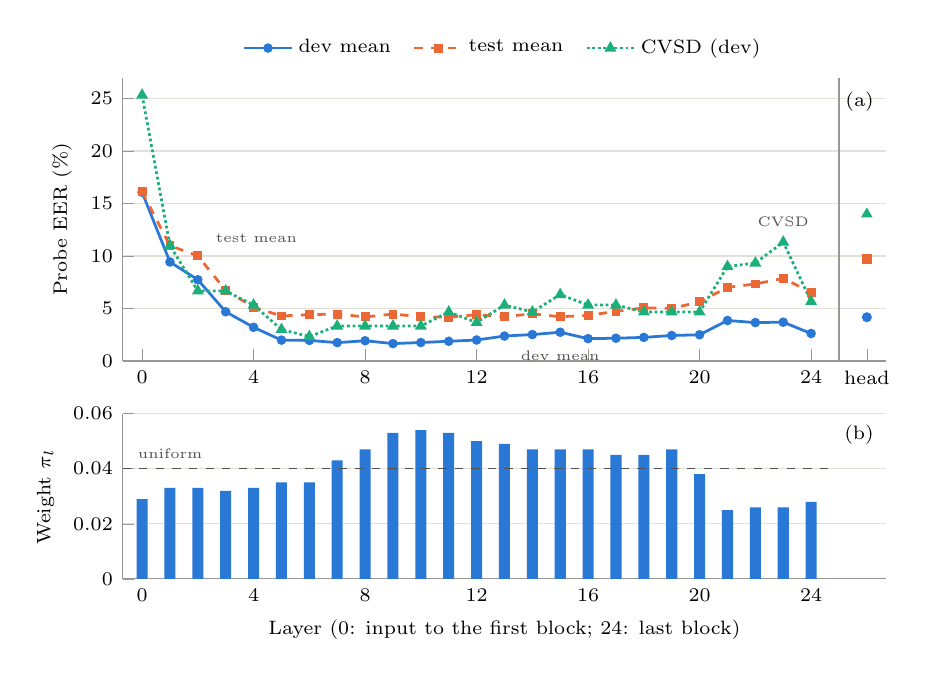
\begin{tikzpicture}
\begin{axis}[
  name=top,
  scale only axis, width=0.80\columnwidth, height=3.6cm,
  xmin=-0.7, xmax=26.7, ymin=0, ymax=27,
  xtick={0,4,8,12,16,20,24,26}, xticklabels={0,4,8,12,16,20,24,head},
  ytick={0,5,10,15,20,25},
  ylabel={Probe EER (\%)},
  tick label style={font=\scriptsize}, label style={font=\scriptsize},
  axis lines*=left, axis line style={inkmuted!60}, tick style={inkmuted!60},
  ymajorgrids, grid style={gridgrey},
  legend style={font=\scriptsize, draw=none, fill=none, at={(0.5,1.03)}, anchor=south, legend columns=3,
    /tikz/every even column/.append style={column sep=6pt}},
  legend cell align=left,
]
\addplot[seriesA, line width=1pt, mark=*, mark size=1.2pt] coordinates {
(0,16.07) (1,9.43) (2,7.74) (3,4.69) (4,3.21) (5,1.99) (6,1.96) (7,1.75) (8,1.93) (9,1.66) (10,1.76) (11,1.88) (12,2.00)
(13,2.38) (14,2.52) (15,2.74) (16,2.13) (17,2.17) (18,2.25) (19,2.43) (20,2.50) (21,3.86) (22,3.66) (23,3.70) (24,2.62)};
\addlegendentry{dev mean}
\addplot[seriesB, line width=1pt, dashed, mark=square*, mark size=1.1pt, mark options={solid}] coordinates {
(0,16.12) (1,10.99) (2,10.01) (3,6.73) (4,5.13) (5,4.29) (6,4.42) (7,4.47) (8,4.20) (9,4.47) (10,4.22) (11,4.18) (12,4.41)
(13,4.24) (14,4.49) (15,4.22) (16,4.34) (17,4.73) (18,5.06) (19,5.01) (20,5.63) (21,7.01) (22,7.34) (23,7.87) (24,6.55)};
\addlegendentry{test mean}
\addplot[seriesC, line width=1pt, densely dotted, mark=triangle*, mark size=1.5pt, mark options={solid}] coordinates {
(0,25.33) (1,11.00) (2,6.67) (3,6.67) (4,5.33) (5,3.00) (6,2.33) (7,3.33) (8,3.33) (9,3.33) (10,3.33) (11,4.67) (12,3.67)
(13,5.33) (14,4.67) (15,6.33) (16,5.33) (17,5.33) (18,4.67) (19,4.67) (20,4.67) (21,9.00) (22,9.33) (23,11.33) (24,5.67)};
\addlegendentry{CVSD (dev)}
% the original detector (its own head on layer 24), shown as separate points
\addplot[seriesA, only marks, mark=*, mark size=1.6pt, forget plot] coordinates {(26,4.17)};
\addplot[seriesB, only marks, mark=square*, mark size=1.5pt, forget plot] coordinates {(26,9.73)};
\addplot[seriesC, only marks, mark=triangle*, mark size=2pt, forget plot] coordinates {(26,14.00)};
\draw[inkmuted!60] (axis cs:25,0) -- (axis cs:25,27);
\node[font=\tiny, text=inkmuted, anchor=south] at (axis cs:23,11.9) {CVSD};
\node[font=\tiny, text=inkmuted, anchor=south west] at (axis cs:2.3,10.4) {test mean};
\node[font=\tiny, text=inkmuted, anchor=north] at (axis cs:15,1.9) {dev mean};
\node[font=\scriptsize, anchor=north east] at (axis cs:26.6,26.6) {(a)};
\end{axis}
% panel (b): its axis box is placed exactly under panel (a), so the layers line up
\begin{axis}[
  at={(top.south west)}, anchor=north west, yshift=-19pt,
  scale only axis, width=0.80\columnwidth, height=2.1cm,
  xmin=-0.7, xmax=26.7, ymin=0, ymax=0.06,
  xtick={0,4,8,12,16,20,24},
  ytick={0,0.02,0.04,0.06}, scaled y ticks=false,
  yticklabel style={/pgf/number format/fixed, /pgf/number format/precision=2},
  xlabel={Layer (0: input to the first block; 24: last block)},
  ylabel={Weight $\pi_l$},
  tick label style={font=\scriptsize}, label style={font=\scriptsize},
  axis lines*=left, axis line style={inkmuted!60}, tick style={inkmuted!60},
  ymajorgrids, grid style={gridgrey},
]
\addplot[ybar, bar width=4pt, fill=seriesA, draw=none] coordinates {
(0,0.029) (1,0.033) (2,0.033) (3,0.032) (4,0.033) (5,0.035) (6,0.035) (7,0.043) (8,0.047) (9,0.053) (10,0.054) (11,0.053) (12,0.050)
(13,0.049) (14,0.047) (15,0.047) (16,0.047) (17,0.045) (18,0.045) (19,0.047) (20,0.038) (21,0.025) (22,0.026) (23,0.026) (24,0.028)};
\draw[inkmuted, dashed] (axis cs:-0.7,0.04) -- (axis cs:24.7,0.04);
\node[font=\tiny, text=inkmuted, anchor=south west] at (axis cs:-0.5,0.04) {uniform};
\node[font=\scriptsize, anchor=north east] at (axis cs:26.6,0.0595) {(b)};
\end{axis}
\end{tikzpicture}
\caption{\textbf{Where the deepfake evidence survives processing (Step 8c).} (a)~EER of a logistic-regression probe on each layer of the frozen detector, trained on clean and processed training views. ``head'': the original detector, whose head reads layer 24. (b)~Weights $\pi_l$ of Equation~\ref{eq:backend}; dashed: uniform weight $1/25$. Both point to the middle blocks.}
\label{fig:layers}
\end{figure}

\textbf{Back-end and fusion.} The back-end alone reached a mean development EER of 1.51\% (best epoch 14), against 4.17\% for the original model. The development EER of the fused score fell from 4.17\% at $w=0$ to 1.98\% at $w=0.4$ and 1.43\% at $w=0.8$; $w=0.85$ was chosen (1.39\%). Table~\ref{tab:backend} gives the unseen test sets. The mean EER over the 13 test sets fell from 9.73\% to 4.05\%, and over the 10 processed sets from 11.36\% to 4.50\%. The largest gains were on premium clones: from 8.2\% to 3.0\% without processing, from 34.0\% to 12.7\% under noise suppression, and from 45.1\% to 16.7\% under Opus, where the AUC rose from 0.589 to 0.890. On the Indian-language clones, CVSD fell from 10.0\% to 4.0\%. In-the-Wild, the set on which every fine-tuning run had lost, stayed at 4.67\% (7.5\% to 7.3\% with noise suppression). On the test sets the back-end alone was slightly better than the fused score (3.62\% against 4.05\%). We still report the fused score, because $w$ was fixed on the development data before the test sets were scored.

\begin{table*}[t]
\centering\small
\caption{\textbf{Frozen-detector back-end (Step 8c) on the unseen test sets of Table~\ref{tab:dsp}.} Original: the detector's own head. Back-end: Equation~\ref{eq:backend} alone. Fused: Equation~\ref{eq:fusion} with $w=0.85$, chosen on the development sets. The processing of these test sets was simulated with the same code as the training views, on unseen speakers and generators.}
\label{tab:backend}
\begin{tabular}{@{}llrrrrr@{}}
\toprule
 & & \multicolumn{3}{c}{\textbf{EER \%}} & \multicolumn{2}{c}{\textbf{AUC}}\\
\cmidrule(lr){3-5}\cmidrule(l){6-7}
\textbf{Test set} & \textbf{Processing} & \textbf{Original} & \textbf{Back-end} & \textbf{Fused} & \textbf{Original} & \textbf{Fused}\\
\midrule
Test speakers (Hindi, Telugu) & clean & 0.0 & 0.0 & 0.0 & 1.000 & 1.000\\
 & phone line (G.711) & 2.0 & 0.0 & 0.0 & 0.995 & 1.000\\
 & noise suppression & 5.0 & 1.3 & 1.3 & 0.988 & 1.000\\
 & spectral subtraction & 1.3 & 0.3 & 0.3 & 0.992 & 1.000\\
 & auto-gain + spectral subtraction & 2.0 & 1.0 & 1.3 & 0.998 & 1.000\\
 & Bluetooth CVSD & 10.0 & 3.3 & 4.0 & 0.953 & 0.991\\
 & Bluetooth mSBC-like & 2.0 & 0.0 & 0.0 & 0.996 & 1.000\\
 & Opus & 4.7 & 0.0 & 1.3 & 0.989 & 1.000\\
\midrule
Premium commercial (ElevenLabs, Kokoro) & clean & 8.2 & 3.4 & 3.0 & 0.956 & 0.989\\
 & noise suppression & 34.0 & 11.2 & 12.7 & 0.699 & 0.946\\
 & Opus & 45.1 & 14.1 & 16.7 & 0.589 & 0.890\\
\midrule
In-the-Wild sample & clean & 4.7 & 4.7 & 4.7 & 0.992 & 0.986\\
 & noise suppression & 7.5 & 7.7 & 7.3 & 0.974 & 0.976\\
\midrule
\textbf{Mean of the 13 test sets} & & \textbf{9.73} & \textbf{3.62} & \textbf{4.05} & & \\
Mean of the 10 processed sets & & 11.36 & 3.90 & 4.50 & & \\
\bottomrule
\end{tabular}
\end{table*}

\textbf{Automatic line profile.} The per-processing thresholds of the original detector confirm the shift seen in Step~8. The EER threshold is $\llr=-3.99$ for the pooled development sets, but $+0.20$ for Opus and $-6.95$ for CVSD; clean audio gives $-4.28$, the phone line $-3.26$ and auto-gain $-5.80$. The processing classifier recognised the processing of the calibration sets with 86.6\% mean accuracy. It reached 80.7--98.0\% on the test speakers and 92.8--98.5\% on processed premium clones, but recognised only 59.5\% of clean premium clips as clean, and it called most In-the-Wild clips Opus, which may be a fair description of compressed internet audio.

Table~\ref{tab:autocal} shows the effect of the automatic threshold. Opus false alarms on genuine Indian-language speech fell from 32.7\% (49 of 150) to 13.3\% (20 of 150; 95\% Wilson interval 8.8--19.7\%) for the original detector, and from 7.3\% to 2.7\% (4 of 150; 1.0--6.7\%) for the fused score, with no more than 2.0\% of fakes missed. CVSD misses of the original detector fell from 26.0\% to 12.0\%. But the errors moved rather than disappeared. False alarms rose on CVSD (1.3\% to 8.7\%) and on auto-gain (3.3\% to 10.0\%), and misses on premium clones under Opus rose from 57.7\% to 78.4\%. Averaged over the 10 processed sets, the half total error rate changed from 13.6\% to 12.9\% for the original detector and from 4.7\% to 5.0\% for the fused score. With the true processing type instead of the predicted one, the results were almost the same, so the classifier is not what limits the method.

\begin{table}[t]
\centering\footnotesize
\caption{\textbf{Automatic line profile (Step 8c): false alarms on genuine speech / missed fakes (\%).} Opus, CVSD and AGC + SS: test speakers. Single: one threshold, the EER threshold of the pooled development sets (Table~\ref{tab:dsp} used a slightly different one, hence 26.0\% instead of 26.7\% CVSD misses). Auto: the threshold of the processing type predicted by the classifier. HTER: half total error rate.}
\label{tab:autocal}
\setlength{\tabcolsep}{3pt}
\begin{tabular}{@{}p{0.21\columnwidth}cccc@{}}
\toprule
 & \multicolumn{2}{c}{\textbf{Original}} & \multicolumn{2}{c}{\textbf{Fused}}\\
\cmidrule(lr){2-3}\cmidrule(l){4-5}
\textbf{Test set} & \textbf{Single} & \textbf{Auto} & \textbf{Single} & \textbf{Auto}\\
\midrule
Opus & 32.7/0.0 & 13.3/2.0 & 7.3/0.0 & 2.7/0.0\\
BT CVSD & 1.3/26.0 & 8.7/12.0 & 3.3/4.7 & 4.0/5.3\\
AGC + SS & 3.3/0.7 & 10.0/0.7 & 2.0/0.0 & 1.3/0.7\\
Premium clones, Opus & 32.6/57.7 & 12.9/78.4 & 12.4/22.4 & 7.3/32.8\\
In-the-Wild & 4.7/5.7 & 3.3/9.7 & 0.7/8.0 & 0.7/9.7\\
\midrule
Mean of 10 processed sets & 8.9/18.2 & 6.8/19.0 & 3.8/5.7 & 3.2/6.7\\
HTER, same sets & 13.6 & 12.9 & 4.7 & 5.0\\
\bottomrule
\end{tabular}
\end{table}

\textbf{In the live server, on real recordings (Step 8d).} We then switched the live server to the fused score and replayed the demo calls and the saved laptop recordings of Section~\ref{sec:mic} through the full pipeline (Table~\ref{tab:live8c}). The exported model gave the original detector's own score to within 0.0003 over 190 real windows and needed about 5\% more CPU time per window (about 340\,ms). The fused score has its own thresholds, set by the same rules as before and never on the demo files. The default is $-1.91$, the pooled development EER. The \texttt{studio} threshold, the window EER on Hume fakes and four development speakers, is 0.00: the development EER fell from 2.1\% to 0.4\%, and the raw EER point lay above the upper limit of 0. The laptop-microphone threshold is $-1.64$, recalibrated with Equation~\ref{eq:calib} on the same two sessions as the original \texttt{mic} profile. Genuine callers stayed at PASS with lower risk under every profile. With the default profiles, the ElevenLabs and Kokoro clones went from VERIFY to HOLD (after 5.6\,s and 13.1\,s). With all 13 ElevenLabs windows above the threshold, against 4 of 13 before. With the \texttt{studio} profiles, the ElevenLabs clone went from VERIFY to HOLD after 12.3\,s, while the Kokoro clone went from a HOLD after 16.5\,s to VERIFY. The strict \texttt{studio} threshold reflects how easy the Hume calibration fakes are for the fused score. In every setting each clone reached at least VERIFY, which the scam rules turn into HOLD when a scam script is used. The processing classifier labelled 38 of 43 windows recorded with the Windows enhancements on as noise suppression, and the raw microphone as clean, so it recognises real device processing. The false alarm it causes, however, was only partly removed: one session dropped from a false HOLD to VERIFY, while the other was still held. The simulated noise suppression used in training does not cover the laptop's combination of noise suppression, beam-forming and gain control.

\begin{table}[t]
\centering\footnotesize
\caption{\textbf{Full pipeline on real recordings, original detector versus Step 8c (Step 8d).} Each detector uses its own profile of the same kind: \texttt{default} / \texttt{studio} for the demo calls, \texttt{mic} for the laptop recordings. V: VERIFY; H $t$: HOLD after $t$ seconds. Enh.: Windows audio enhancements.}
\label{tab:live8c}
\setlength{\tabcolsep}{3pt}
\begin{tabular}{@{}p{0.30\columnwidth}p{0.31\columnwidth}p{0.31\columnwidth}@{}}
\toprule
\textbf{Recording} & \textbf{Original} & \textbf{Step 8c}\\
\midrule
Genuine caller 1 / 2 & PASS / PASS & PASS / PASS\\
ElevenLabs clone & V / V & H 5.6 / H 12.3\\
Kokoro clone & V / H 16.5 & H 13.1 / V\\
Scam call, Windows TTS & H 4.4 / H 4.4 & H 4.4 / H 4.4\\
\midrule
Laptop mic, enh. on, session 1 & false HOLD & VERIFY\\
Laptop mic, enh. on, session 2 & false HOLD (6.2 s) & false HOLD (15.8 s)\\
\bottomrule
\end{tabular}
\end{table}

\subsection{Attack with a Clone of the Enrolled Person (Step 9)}
\label{sec:attack}
The hardest case for the voiceprint check is a clone of the very person the caller claims to be.

\textbf{The clone.} We made one locally with kNN-VC (Baas et al., 2023), with the team member's consent:
\begin{itemize}\setlength\itemsep{0pt}
\item the target voice came from 119\,s of the enrolled team member's own laptop recordings;
\item the clone reads the bank-fraud script of the demo.
\end{itemize}
We ran it through the full pipeline with that identity claimed (Table~\ref{tab:attack}).

\textbf{Offline.} The voiceprint similarity of the clone was 0.41, close to the cut-off of 0.45 (the genuine speaker scored 0.95). The identity check alone therefore nearly accepted it. The AI-voice detector flagged all 18 windows, with both the original detector and Step 8c. Together with the scam rules, the call reached HOLD after 4.4\,s.

\textbf{Through a live call.} We played the clone into a WebRTC call in two automated runs of the call demonstrator.
\begin{itemize}\setlength\itemsep{0pt}
\item The call reached VERIFY after 3.8--4.5\,s, because the voice did not match the claimed person. The call channel lowered the mean similarity to 0.32.
\item It reached HOLD after 7.8--10.0\,s.
\item The Rs.~49,999 transfer requested during the call was blocked automatically.
\end{itemize}

\textbf{Limits of this test.} The clone is an open-source one made from two minutes of speech. A premium clone of the enrolled person has not been tested.

\begin{table}[t]
\centering\footnotesize
\caption{\textbf{Attack with a clone of the enrolled person (Step 9).} The caller claims to be the enrolled team member. Similarity: mean voiceprint cosine (cut-off 0.45). Offline rows use the full pipeline with Step 8c; call rows are two automated runs of the two-window demonstrator.}
\label{tab:attack}
\setlength{\tabcolsep}{3pt}
\begin{tabular}{@{}p{0.34\columnwidth}p{0.14\columnwidth}p{0.17\columnwidth}p{0.27\columnwidth}@{}}
\toprule
\textbf{Caller} & \textbf{Similarity} & \textbf{Detector} & \textbf{Verdict}\\
\midrule
Clone of the enrolled person + scam script, offline & 0.41 & 18/18 windows & HOLD at 4.4 s\\
Same clone through the WebRTC call & 0.32--0.33 & median score 13 & VERIFY 3.8--4.5 s, HOLD 7.8--10.0 s, transfer blocked\\
Enrolled person's real voice, offline & 0.95 & 0/19 windows & PASS\\
Robot-voice scam script, offline & $-0.06$ & 18/18 windows & HOLD at 4.4 s\\
\bottomrule
\end{tabular}
\end{table}

\subsection{Software Quality}
\label{sec:tests}
The server has 41 fast tests with stubbed models and 9 tests with the real models, all passing. They cover the resampler, VAD windowing, invariance to the chunk size, risk escalation, calibration rules, multilingual scam tactics, the voiceprint store, utterance cutting, the WebSocket flows (genuine, cloned, 44.1\,kHz input, calibration, enrolment, claimed identity, invalid start), the signalling relay (join, offer and answer relay, peer left, invalid role refused), the prevention-event interface and the web pages. The real-model tests check that voiceprints separate two real speakers, that the scam call reaches HOLD with ``asks for OTP'', and that the Step 8c model reproduces the original detector's score and gives the expected verdicts on the demo calls. Every Kaggle notebook is first run end to end on the CPU with stub data and weights of the real shapes, including LoRA training, merging and ONNX export (difference between ONNX and PyTorch outputs below $10^{-4}$), because a failed GPU run costs hours of queue time. For Step 8c the same test also checks the serving path: the ONNX layer outputs and the NumPy back-end reproduce the notebook's features and fused scores.

\subsection{Defects Found and Fixed}
Table~\ref{tab:defects} lists the main defects. Several produced plausible output and were found only by comparing numbers across runs, devices or recordings.

\begin{table*}[t]
\centering\footnotesize
\caption{\textbf{Defects found during development.}}
\label{tab:defects}
\begin{tabular}{@{}p{0.29\textwidth}p{0.33\textwidth}p{0.30\textwidth}@{}}
\toprule
\textbf{Defect} & \textbf{Effect} & \textbf{Fix}\\
\midrule
Baseline classifier evaluated on its own training data & 1.3\% EER that means nothing & excluded; only unseen sets reported\\
kNN-VC clones cleaner than genuine clips & risk of learning ``clean means fake'' & identical augmentation for both classes\\
Small-data fine-tuning (Steps 4 and 8) & forgetting of real-world fakes & selection on unseen dev sets with the original as step 0; frozen detector with a small back-end (Step 8c)\\
Browser default input was a Bluetooth headset or virtual mixer & genuine voice at $\llr=+2.2$, false HOLD & explicit microphone choice, level meter, ``no Bluetooth'' rule\\
Windows microphone enhancements & genuine voice at $-2.3$, false HOLD, unstable across sessions & enhancements off; \texttt{mic} profile recalibrated on raw audio\\
Running risk started at the first window & one odd window gave VERIFY & running risk starts at 0 (genuine)\\
Line profile reset after a page reload & wrong threshold in a live test & profile remembered in the browser\\
Resampler off by one sample, weak anti-aliasing & small score differences with chunk size & corrected; elliptic filter; chunk-size test\\
Whisper on GPU missing a CUDA library & transcription failed or fell back to CPU & NVIDIA libraries from pip, explicit DLL path\\
Kaggle: new PEFT refused an old pre-installed torchao & notebook crashed at import & torchao removed in the install cell\\
ONNX export of a dynamic layer norm & export failed & explicit mean and variance in a wrapper; weight-norm removed before export\\
Newer Transformers library returns the last hidden layer \emph{before} the final layer norm & cached last-layer features no longer reproduced the detector (score off by 0.13) & last layer taken from the model's final output; the notebook asserts that the head reproduces the detector\\
Detector slow while the laptop is busy & 1--8 s per window instead of 0.33 s & close heavy applications; GPU detector planned\\
Scam keyword in an innocent story (``drugs'') & scam score 40 on a genuine call & below the alert level; scam words alone never give HOLD\\
\bottomrule
\end{tabular}
\end{table*}

% =====================================================================
\FloatBarrier
\section{Discussion}
\textbf{The detector is good, the channel is the problem.} Zero-shot, the post-trained SSL detector handled open-source clones in Hindi and Telugu and real-world English deepfakes. Its failures came from two directions: premium commercial voices, and processing between the speaker and the detector. The second is more serious for a deployed system, because the same processing affects genuine callers. A wrong input device or the operating-system enhancements moved a genuine voice from $\llr=-10$ to $-2$ or even $+2$, which is a larger shift than the difference between our own voice and a premium AI voice ($-10.3$ against $-4.6$). In our experience this is the most practical lesson of the project: a detector threshold is only meaningful for a known input chain, and that chain has to be fixed, measured and calibrated.

\textbf{Shift, loss or read-out.} Table~\ref{tab:dsp} first suggested two kinds of damage. Opus on Indian-language speech mainly \emph{shifts} the scores (EER 4.7\%, but 32.7\% false alarms at the old threshold), and a per-processing threshold corrects part of that (Table~\ref{tab:autocal}). Noise suppression and Opus on premium clones brought the AUC of the original detector down to 0.70 and 0.59, which looked like a \emph{loss} of the evidence. Step 8c shows that this reading was only partly right. The frozen representation still separates these clips (AUC 0.95 and 0.92 for the back-end), so most of the evidence survives, mainly in the middle blocks, and is lost by the read-out. Some loss remains (EER 11--17\%), and it may be larger for real codecs and real noise suppression than for our simulations.

\textbf{Why fusion matters.} The detector alone gave a premium clone VERIFY rather than HOLD. The voiceprint was decisive when the voice did not belong to the claimed person (similarity 0.0--0.1 against 0.82), and the scam rules turn a suspicious voice plus a scam script into HOLD. The rules are deliberately asymmetric: a matching voice never lowers the risk, scam words from a genuine voice give VERIFY only, and the verdict never de-escalates.

\textbf{Negative fine-tuning results.} Three fine-tuning runs (full fine-tuning in Step~4, LoRA with the label loss only, and LoRA with the teacher-anchored consistency loss in Step~8) all improved some of the conditions they were trained on and damaged others, above all real-world fakes. All three were rejected because the original model was a candidate in model selection and the development sets included unseen generators and real-world fakes. The consistency anchor did not change the outcome. Our reading is that the anchor only constrains the model on the training distribution (Indian-language speech and commercial TTS); nothing holds its behaviour in place on In-the-Wild-like audio, which drifted in the same way as without the anchor. A second factor may be the label loss itself: it is computed at $p_{\text{fake}}=0.5$, whereas the model's calibrated threshold is 0.0185, and the high starting cross-entropy (1.6) suggests that much of the training effort goes into moving the decision boundary towards the training domain rather than into robustness. With about 4k clips against 74k hours of post-training, changing the detector's weights did not work in our hands. Without model selection on unseen sets we would have shipped worse models; our two earlier attempts before this project, a spectrogram CNN and a wav2vec~2.0 classifier trained from a general checkpoint, had no such safeguard.

\textbf{Why the frozen back-end works.} Step 8c suggests that the weights did not need to change. The probes show that the evidence was already in the frozen representation, and the back-end reads it with 1,050 parameters instead of 3.54\,M. Since the backbone is fixed, its behaviour on audio unlike the training data cannot drift, and In-the-Wild stayed at 4.67\%. The original head remains part of the fused score and was always a candidate during selection ($w=0$). That the middle blocks are the most robust fits the observation that the upper blocks of wav2vec~2.0 are shaped most by the training objective and change most when the model is fine-tuned (Pasad et al., 2021). In our detector, the upper blocks were post-trained to read deepfake cues from audio without consumer processing. The improvement on clean premium clones (8.2\% to 3.0\%), whose generators were never seen in training, shows that the back-end did not only learn our processing simulations. The processed test sets, however, used the same simulation code as the training views, so the size of the gains there is an upper bound for real devices. The live check confirms this. The real premium clone was caught much better, but the laptop's own noise suppression still caused a false alarm in one of two sessions.

\textbf{Thresholds cannot replace a better score.} The automatic line profile removes most of the Opus shift without manual configuration, but it moved errors between false alarms and misses rather than reducing them: the half total error rate barely changed. A threshold can only choose a point on a fixed trade-off; the back-end changes the trade-off itself. With the fused score, a single threshold was already as good as the automatic one. We therefore see the automatic profile as an option for lines where Opus false alarms matter, not as the main fix.

\textbf{Mapping to the problem statement.} Table~\ref{tab:sih} maps the requirements of SIH26104 to the implementation and states what is not done.

\begin{table}[t]
\centering\footnotesize
\caption{\textbf{Requirements of SIH26104 and their status.}}
\label{tab:sih}
\begin{tabular}{@{}p{0.31\columnwidth}p{0.59\columnwidth}@{}}
\toprule
\textbf{Requirement} & \textbf{Status}\\
\midrule
Acoustic analysis for synthesis artefacts & SSL detector on 4 s windows every second, with the Step 8c layer back-end; done\\
Checks against genuine samples & voiceprint enrolment and running mismatch; done\\
Real-time risk engine, configurable thresholds & explainable rules, line profiles per score, configuration file, optional automatic per-processing threshold; done\\
Prosody and behaviour modelling & not implemented\\
Context (transaction, call origin) & transaction in the bank app; call origin and contacts not used\\
Alerts and pre-transaction prompts & in-app alerts, webhook, OTP or call-back, automatic block; SMS is simulated\\
Privacy & no audio, transcripts or voiceprints in logs; inference on the laptop; voiceprints deletable\\
Interfaces & REST and WebSocket; no SDK or gRPC\\
Multilingual, Indian accents & Hindi and Telugu tested for the detector; scam rules in English, Hindi and Telugu; Whisper weaker on Telugu\\
\bottomrule
\end{tabular}
\end{table}

\textbf{Responsible use and privacy.} VoiceShield produces warnings and starts bank-side checks; a human decides. The audit log stores scores, decisions and tactic names only. Recordings of team members were made with their consent, and no third person's voice was cloned. The detector licence (CC BY-NC-SA) and the IndicSynth licence (CC BY-NC) restrict the work to non-commercial use.

\textbf{Threats to validity.} \emph{Internal:} the test sets have 150 to a few hundred clips per class, so differences of one or two points are within sampling noise; the live tests are single sessions; the \texttt{mic} profile was calibrated on two sessions of one speaker. In Step 8c the back-end epoch and the fusion weight were chosen on the development sets, so the development numbers are optimistic; only the test sets are free of selection. \emph{Construct:} our DSP effects are simulations; real noise suppression in phones and calling apps differs, and our mSBC channel is an approximation. The Step 8c back-end was trained on views processed by the same simulation code as the processed test sets (with other speakers, generators and random draws), so its gains there measure robustness to our simulations; the unseen premium generators and the In-the-Wild sample are the stronger evidence. \emph{External:} the premium clones in the offline tests come from two commercial systems; the live tests used one laptop, one microphone and one premium voice; Indian-language clones were made with kNN-VC and the IndicSynth generators only.

\textbf{Limitations.}
\label{sec:limits}
(i) A good clone \emph{of the enrolled person} can pass the voiceprint check: our open-source clone came within 0.04 of the cut-off, and the voiceprint mainly targets human impersonators and clones of someone else. (ii) An open-source clone of the enrolled person was held through the call (Section~\ref{sec:attack}), but a premium clone of the enrolled person through the call remains untested. (iii) Genuine-caller and human-impersonator scenarios through the call, and a calibrated profile for the call channel, still need live microphones. (iv) The scam rules are keyword based and can fire on innocent words. (v) The demonstrator uses a WebRTC call, not a cellular call. (vi) The detector slows down on a busy laptop. (vii) Three fine-tuning runs have not improved the detector. The frozen-detector back-end did, but it was measured mainly on simulated processing. On real audio it was checked only on the demo calls and on four laptop sessions of one speaker, and the laptop's own noise suppression still caused one false alarm, so the enhancements must stay off.

\textbf{Future work.}
\label{sec:future}
The back-end now runs in the live server. Its training views should next include real device processing: recordings through operating-system enhancements, Bluetooth headsets and VoIP applications, and re-recorded corpora such as RTCFake (Xue et al., 2026). These would show how much of the gain carries over, and they target the false alarm that the laptop's noise suppression still causes. The back-end itself could pool over time with attention instead of the mean, or use more training generators. Beyond the model: an attack test with a clone of the enrolled person and premium clones through the call; a calibrated call-channel profile; the detector on the GPU; a phone as the caller over HTTPS; a learned scam classifier for Hinglish; and a larger, multi-speaker live evaluation.

\section{Conclusion}
We built VoiceShield, a real-time system that fuses a synthetic-voice detector, a voiceprint check and scam-language rules into an explainable PASS/VERIFY/HOLD decision and blocks a payment when a call is judged an impersonation. A post-trained SSL detector worked zero-shot on Indian-language clones and real-world deepfakes, and our own fine-tuning did not beat it, which we report as a negative result. In live tests a premium AI voice was held after 5.3\,s while the same script read by a person passed, and an injected scam call was held after about 4\,s of speech with the transfer blocked. Our main finding is that consumer audio processing, from operating-system microphone enhancements to noise suppression and VoIP codecs, can turn a genuine voice into a false alarm and make premium clones nearly undetectable. Two parameter-efficient fine-tuning methods, one of them anchored to the original model, learned the processed conditions but lost accuracy on real-world fakes and were rejected by model selection. Keeping the detector frozen worked better. Layer-wise probes showed that the evidence survives processing mainly in the middle blocks and that much of the damage is in the read-out. A 1,050-parameter back-end fused with the original head reduced the mean EER over 13 unseen test sets from 9.7\% to 4.1\%, including premium clones under Opus from 45.1\% to 16.7\%, without any loss on real-world deepfakes. An automatic per-processing threshold removed most of the Opus false alarms but only moved errors overall. In the live server, with the default thresholds, the back-end turned two premium clones that had only reached VERIFY into HOLDs, without false alarms on genuine callers. It did not fully remove the false alarms caused by the laptop's own noise suppression, so a deployed detector must still control and calibrate its input chain. A clone of the enrolled person nearly passed the voiceprint check but was caught by the detector in every window. That case shows why the decision should rest on several independent signals.

% =====================================================================
\section{Author Contributions}
% CHECK and complete for every author.
A.A.C. defined the system, the risk policy and the evaluation, ran the Kaggle experiments and the live tests, recorded the calibration and test audio, reviewed the results and edited the manuscript.

\section{Use of AI Tools}
An AI coding assistant (Claude Code) implemented most of the server, the web pages, the Kaggle notebooks and the test suites from the authors' requirements, and prepared a first draft of this manuscript from the project's results log. The authors ran every experiment, checked the printed evidence (notebook outputs, test results, live recordings), found several of the defects in Table~\ref{tab:defects} this way, and revised the text. ChatGPT's voice mode was used as a premium synthetic voice in the live tests.

\section{Acknowledgments}
We thank Lovely Professional University for guidance and support, and the authors of the AntiDeepfake, WeSpeaker, Silero VAD, Whisper, Kathbath, IndicSynth and In-the-Wild resources for releasing them.

\section{Data and Code Availability}
The code, the Kaggle notebooks, the results log and the figures are available at \url{https://github.com/AlapatiAbhinavChowdhary/VoiceShield}. The large model files are downloaded by a setup script. The public data sets can be obtained from their publishers under their licences. Our own voice recordings and voiceprints are not released.

\begin{thebibliography}{50}
\setlength{\itemsep}{2pt}
\bibitem[Baas et~al.(2023)]{baas2023} Baas, M., van Niekerk, B., and Kamper, H. (2023). Voice conversion with just nearest neighbors. In \emph{Proceedings of Interspeech 2023}, 2053--2057.
\bibitem[Babu et~al.(2022)]{babu2022} Babu, A., Wang, C., Tjandra, A., Lakhotia, K., Xu, Q., Goyal, N., et al. (2022). XLS-R: Self-supervised cross-lingual speech representation learning at scale. In \emph{Proceedings of Interspeech 2022}, 2278--2282.
\bibitem[Baevski et~al.(2020)]{baevski2020} Baevski, A., Zhou, Y., Mohamed, A., and Auli, M. (2020). wav2vec 2.0: A framework for self-supervised learning of speech representations. In \emph{Advances in Neural Information Processing Systems (NeurIPS)}, vol.~33, 12449--12460.
\bibitem[Boll(1979)]{boll1979} Boll, S. (1979). Suppression of acoustic noise in speech using spectral subtraction. \emph{IEEE Transactions on Acoustics, Speech, and Signal Processing} 27(2), 113--120.
\bibitem[Brown et~al.(2001)]{brown2001} Brown, L. D., Cai, T. T., and DasGupta, A. (2001). Interval estimation for a binomial proportion. \emph{Statistical Science} 16, 101--133.
\bibitem[Chandra et~al.(2025)]{chandra2025} Chandra, N. A., Murtfeldt, R., Qiu, L., Karmakar, A., Lee, H., Tanumihardja, E., et al. (2025). Deepfake-Eval-2024: A multi-modal in-the-wild benchmark of deepfakes circulated in 2024. \emph{arXiv preprint arXiv:2503.02857}.
\bibitem[Desplanques et~al.(2020)]{desplanques2020} Desplanques, B., Thienpondt, J., and Demuynck, K. (2020). ECAPA-TDNN: Emphasized channel attention, propagation and aggregation in TDNN based speaker verification. In \emph{Proceedings of Interspeech 2020}, 3830--3834.
\bibitem[Ge et~al.(2025)]{ge2025} Ge, W., Wang, X., Liu, X., and Yamagishi, J. (2025). Post-training for deepfake speech detection. In \emph{Proceedings of the IEEE Automatic Speech Recognition and Understanding Workshop (ASRU)}. arXiv:2506.21090. Model: \url{https://huggingface.co/nii-yamagishilab/wav2vec-large-anti-deepfake}.
\bibitem[Hinton et~al.(2015)]{hinton2015} Hinton, G., Vinyals, O., and Dean, J. (2015). Distilling the knowledge in a neural network. \emph{arXiv preprint arXiv:1503.02531}.
\bibitem[Hu et~al.(2022)]{hu2022} Hu, E. J., Shen, Y., Wallis, P., Allen-Zhu, Z., Li, Y., Wang, S., Wang, L., and Chen, W. (2022). LoRA: Low-rank adaptation of large language models. In \emph{International Conference on Learning Representations (ICLR)}.
\bibitem[ITU-T(1988)]{itu1988} ITU-T (1988). \emph{Recommendation G.711: Pulse code modulation (PCM) of voice frequencies}. International Telecommunication Union.
\bibitem[Javed et~al.(2023)]{javed2023} Javed, T., Bhogale, K., Raman, A., Kumar, P., Kunchukuttan, A., and Khapra, M. M. (2023). IndicSUPERB: A speech processing universal performance benchmark for Indian languages. In \emph{Proceedings of the AAAI Conference on Artificial Intelligence} 37(11), 12942--12950.
\bibitem[Jung et~al.(2022a)]{jung2022sasv} Jung, J.-w., Tak, H., Shim, H.-j., Heo, H.-S., Lee, B.-J., Chung, S.-W., et al. (2022a). SASV 2022: The first spoofing-aware speaker verification challenge. In \emph{Proceedings of Interspeech 2022}, 2893--2897.
\bibitem[Jung et~al.(2022b)]{jung2022aasist} Jung, J.-w., Heo, H.-S., Tak, H., Shim, H.-j., Chung, J. S., Lee, B.-J., Yu, H.-J., and Evans, N. (2022b). AASIST: Audio anti-spoofing using integrated spectro-temporal graph attention networks. In \emph{Proceedings of ICASSP 2022}, 6367--6371.
\bibitem[Kawa et~al.(2023)]{kawa2023} Kawa, P., Plata, M., Czuba, M., Szyma\'nski, P., and Syga, P. (2023). Improved DeepFake detection using Whisper features. In \emph{Proceedings of Interspeech 2023}, 4009--4013.
\bibitem[Kirkpatrick et~al.(2017)]{kirkpatrick2017} Kirkpatrick, J., Pascanu, R., Rabinowitz, N., Veness, J., Desjardins, G., Rusu, A. A., et al. (2017). Overcoming catastrophic forgetting in neural networks. \emph{Proceedings of the National Academy of Sciences} 114(13), 3521--3526.
\bibitem[Li and Hoiem(2018)]{li2018} Li, Z., and Hoiem, D. (2018). Learning without forgetting. \emph{IEEE Transactions on Pattern Analysis and Machine Intelligence} 40(12), 2935--2947.
\bibitem[Liu et~al.(2023)]{liu2023} Liu, X., Wang, X., Sahidullah, M., Patino, J., Delgado, H., Kinnunen, T., et al. (2023). ASVspoof 2021: Towards spoofed and deepfake speech detection in the wild. \emph{IEEE/ACM Transactions on Audio, Speech, and Language Processing} 31, 2507--2522.
\bibitem[Luong et~al.(2026)]{luong2026} Luong, H.-T., Liu, X., Kukanov, I., Chai, Z. X., and Lee, K. A. (2026). RADAR Challenge 2026: Robust audio deepfake recognition under media transformations. \emph{arXiv preprint arXiv:2605.09568}.
\bibitem[M\"uller et~al.(2021)]{muller2021} M\"uller, N. M., Dieckmann, F., Czempin, P., Canals, R., B\"ottinger, K., and Williams, J. (2021). Speech is silver, silence is golden: What do ASVspoof-trained models really learn? In \emph{Proceedings of the ASVspoof 2021 Workshop}, 55--60.
\bibitem[M\"uller et~al.(2022)]{muller2022} M\"uller, N. M., Czempin, P., Dieckmann, F., Froghyar, A., and B\"ottinger, K. (2022). Does audio deepfake detection generalize? In \emph{Proceedings of Interspeech 2022}, 2783--2787.
\bibitem[Nagrani et~al.(2017)]{nagrani2017} Nagrani, A., Chung, J. S., and Zisserman, A. (2017). VoxCeleb: A large-scale speaker identification dataset. In \emph{Proceedings of Interspeech 2017}, 2616--2620.
\bibitem[Pasad et~al.(2021)]{pasad2021} Pasad, A., Chou, J.-C., and Livescu, K. (2021). Layer-wise analysis of a self-supervised speech representation model. In \emph{Proceedings of the IEEE Automatic Speech Recognition and Understanding Workshop (ASRU)}, 914--921.
\bibitem[Radford et~al.(2023)]{radford2023} Radford, A., Kim, J. W., Xu, T., Brockman, G., McLeavey, C., and Sutskever, I. (2023). Robust speech recognition via large-scale weak supervision. In \emph{Proceedings of the 40th International Conference on Machine Learning (ICML)}, 28492--28518.
\bibitem[Sainburg et~al.(2020)]{sainburg2020} Sainburg, T., Thielk, M., and Gentner, T. Q. (2020). Finding, visualizing, and quantifying latent structure across diverse animal vocal repertoires. \emph{PLoS Computational Biology} 16(10), e1008228. Software: noisereduce.
\bibitem[San Roman et~al.(2024)]{sanroman2024} San Roman, R., Fernandez, P., D\'efossez, A., Furon, T., Tran, T., and Elsahar, H. (2024). Proactive detection of voice cloning with localized watermarking. In \emph{Proceedings of the 41st International Conference on Machine Learning (ICML)}.
\bibitem[Sharma et~al.(2025)]{sharma2025} Sharma, D. V., Ekbote, V., and Gupta, A. (2025). IndicSynth: A large-scale multilingual synthetic speech dataset for low-resource Indian languages. In \emph{Proceedings of the 63rd Annual Meeting of the Association for Computational Linguistics (ACL)}, 22037--22060. Data: \url{https://huggingface.co/datasets/vdivyasharma/IndicSynth}.
\bibitem[Silero Team(2024)]{silero2024} Silero Team (2024). Silero VAD: pre-trained enterprise-grade voice activity detector. \url{https://github.com/snakers4/silero-vad}.
\bibitem[Smart India Hackathon(2026)]{sih2026} Smart India Hackathon (2026). Problem statement SIH26104: AI-powered real-time detection and prevention of voice cloning impersonation attacks. AICTE Cyber Security Cell, Government of India. \url{https://www.sih.gov.in}.
\bibitem[Stafford(2025)]{stafford2025} Stafford, G. (2025). Deepfake audio detection data set (ElevenLabs, Polly, Hume, Speechify, Kokoro and real speech). \url{https://huggingface.co/datasets/garystafford/deepfake-audio-detection}.
\bibitem[Tak et~al.(2022a)]{tak2022a} Tak, H., Todisco, M., Wang, X., Jung, J.-w., Yamagishi, J., and Evans, N. (2022a). Automatic speaker verification spoofing and deepfake detection using wav2vec 2.0 and data augmentation. In \emph{Proceedings of Odyssey 2022: The Speaker and Language Recognition Workshop}, 112--119.
\bibitem[Tak et~al.(2022b)]{tak2022b} Tak, H., Kamble, M., Patino, J., Todisco, M., and Evans, N. (2022b). RawBoost: A raw data boosting and augmentation method applied to automatic speaker verification anti-spoofing. In \emph{Proceedings of ICASSP 2022}, 6382--6386.
\bibitem[Valin et~al.(2012)]{valin2012} Valin, J.-M., Vos, K., and Terriberry, T. (2012). \emph{Definition of the Opus Audio Codec}. RFC 6716, Internet Engineering Task Force.
\bibitem[W3C(2021)]{w3c2021} W3C (2021). \emph{WebRTC 1.0: Real-Time Communication Between Browsers}. W3C Recommendation.
\bibitem[Wang et~al.(2020)]{wang2020} Wang, X., Yamagishi, J., Todisco, M., Delgado, H., Nautsch, A., Evans, N., et al. (2020). ASVspoof 2019: A large-scale public database of synthesized, converted and replayed speech. \emph{Computer Speech \& Language} 64, 101114.
\bibitem[Wang et~al.(2024)]{wang2024} Wang, X., Delgado, H., Tak, H., Jung, J.-w., Shim, H.-j., Todisco, M., et al. (2024). ASVspoof 5: Crowdsourced speech data, deepfakes, and adversarial attacks at scale. In \emph{Proceedings of the ASVspoof 2024 Workshop}.
\bibitem[Wang et~al.(2023)]{wang2023} Wang, H., Liang, C., Wang, S., Chen, Z., Zhang, B., Xiang, X., Deng, Y., and Qian, Y. (2023). WeSpeaker: A research and production oriented speaker embedding learning toolkit. In \emph{Proceedings of ICASSP 2023}.
\bibitem[Wilson(1927)]{wilson1927} Wilson, E. B. (1927). Probable inference, the law of succession, and statistical inference. \emph{Journal of the American Statistical Association} 22, 209--212.
\bibitem[Xue et~al.(2026)]{xue2026} Xue, J., Yi, Z., Huang, Y., Ren, Y., Chen, Y., Fan, C., et al. (2026). RTCFake: Speech deepfake detection in real-time communication. In \emph{Findings of the Association for Computational Linguistics: ACL 2026}, 5763--5775.
\bibitem[Yang et~al.(2021)]{yang2021} Yang, S.-w., Chi, P.-H., Chuang, Y.-S., Lai, C.-I. J., Lakhotia, K., Lin, Y. Y., et al. (2021). SUPERB: Speech processing Universal PERformance Benchmark. In \emph{Proceedings of Interspeech 2021}, 1194--1198.
\bibitem[Yu et~al.(2023)]{yu2023} Yu, Z., Zhai, S., and Zhang, N. (2023). AntiFake: Using adversarial audio to prevent unauthorized speech synthesis. In \emph{Proceedings of the ACM SIGSAC Conference on Computer and Communications Security (CCS)}, 460--474.
\bibitem[Zhang et~al.(2024)]{zhang2024} Zhang, Q., Wen, S., and Hu, T. (2024). Audio deepfake detection with self-supervised XLS-R and SLS classifier. In \emph{Proceedings of the 32nd ACM International Conference on Multimedia}, 6765--6773.
\end{thebibliography}

% =====================================================================
\appendix
\onecolumn
\section{Appendix A: Scam Tactics}
Each tactic has a weight $w_k$ in Equation~\ref{eq:scam}. Patterns exist for English, romanised Hindi and Telugu, and Devanagari and Telugu script (not shown).

\begin{table}[H]
\centering\small
\caption{\textbf{Scam-language tactics and weights.}}
\label{tab:tactics}
\begin{tabular}{@{}p{0.30\textwidth}rp{0.52\textwidth}@{}}
\toprule
\textbf{Tactic} & \textbf{$w_k$} & \textbf{Example phrases (English and romanised)}\\
\midrule
Asks for OTP, PIN or password & 0.60 & OTP, one-time password, CVV, UPI PIN, card details, ``OTP batao''\\
Asks to install a remote-access app & 0.50 & AnyDesk, TeamViewer, screen share, APK, ``app install karo''\\
Asks to send or transfer money & 0.40 & transfer, UPI, processing fee, refund, ``paise bhejo'', ``dabbu pampandi''\\
Threatens police, arrest or legal action & 0.40 & police, CBI, customs, digital arrest, warrant, parcel, drugs, FIR\\
Says an account, SIM or KYC will be blocked & 0.35 & account blocked, KYC, SIM suspended, ``khata band''\\
Claims an emergency or accident & 0.35 & accident, hospital, in trouble, need money urgently, ``musibat''\\
Promises a prize, cashback or lottery & 0.30 & lottery, won a prize, cashback, jackpot\\
Pressure to act fast or keep it secret & 0.25 & urgent, within 30 minutes, don't tell anyone, stay on the line, ``jaldi''\\
Claims to be a bank or an official & 0.20 & from your bank, SBI, RBI, customer care, fraud department\\
\bottomrule
\end{tabular}
\end{table}

\section{Appendix B: System Configuration}
\begin{table}[H]
\centering\small
\caption{\textbf{Main settings of the system.}}
\label{tab:config}
\begin{tabular}{@{}p{0.32\textwidth}p{0.58\textwidth}@{}}
\toprule
\textbf{Item} & \textbf{Value}\\
\midrule
Audio & 16 kHz mono; client chunks of about 100 ms; streaming resampler with elliptic anti-aliasing filter\\
VAD & Silero VAD v5, 32 ms frames, threshold 0.5, hangover 300 ms\\
Detector window & 4.0 s of speech (64,000 samples), 1 s hop, first decision after 2 s of speech\\
Line thresholds on $\llr$ & \texttt{default} $-4.07$; \texttt{studio} $-5.63$; \texttt{mic} $-6.01$ (laptop microphone, enhancements off, 2 sessions)\\
Calibration rule (genuine only) & 95th percentile of genuine window scores + 1.5, clipped to $[-9.5, 0]$\\
Risk engine & EMA $\alpha=0.4$ from 0; VERIFY at 45 or 2 of 5 windows; HOLD at 75 with 3 of 5 windows; identity at 50; scam at 50\\
Voiceprint & WeSpeaker ResNet34-LM, 80-band filterbank; enrolment at least 5 windows (about 7 s); $\tau_s=0.45$, $\beta=0.08$\\
Speech recognition & faster-whisper small on GPU (base on CPU); utterances 0.6--8 s; hallucination filter\\
Call & WebRTC, Opus mono 128 kbit/s without DTX; signalling relayed by the server\\
Audit log & SQLite; scores, decisions, tactic names, prevention events; no audio, no transcripts\\
\bottomrule
\end{tabular}
\end{table}

\section{Appendix C: Training Settings}
\begin{table}[H]
\centering\small
\caption{\textbf{Training experiments.} Steps 4, 8 and 8b change the detector's weights; Step 8c keeps the detector frozen.}
\label{tab:train}
\begin{tabular}{@{}p{0.14\textwidth}p{0.17\textwidth}p{0.17\textwidth}p{0.19\textwidth}p{0.21\textwidth}@{}}
\toprule
\textbf{Item} & \textbf{Step 4 (full)} & \textbf{Step 8 (LoRA, attempt 1)} & \textbf{Step 8b (LoRA, attempt 2)} & \textbf{Step 8c (frozen detector)}\\
\midrule
Trainable parameters & all except CNN front end & 3.54 M (1.11\%) & 3.54 M (1.11\%) & 1,050 (back-end) and 9,250 (processing classifier)\\
Training clips & 3,760 & 4,360 & 4,360 & 4,360, three views each (13,080)\\
Loss & cross-entropy & cross-entropy & cross-entropy + gated consistency (Eq.~\ref{eq:consistency}) & binary and 9-class cross-entropy\\
Learning rate & $5\times10^{-6}$ backbone, $5\times10^{-5}$ head & $10^{-4}$ LoRA, $10^{-5}$ head & $5\times10^{-5}$ LoRA, $10^{-5}$ head & $10^{-3}$, batch 256, dropout 0.2\\
Augmentation & noise, denoise, phone, low-pass (both classes) & noise, 7 consumer effects, low-pass (both classes) & processed copy of the same crop in 85\% of clips & 1 clean and 2 processed views (8 processing types)\\
Model selection & mean EER of 4 dev sets & mean EER of 8 dev sets & mean EER of 8 dev sets & mean EER of 8 dev sets (epoch and fusion weight)\\
Early stopping & 4 evaluations & 4 evaluations & 6 evaluations & best of 30 epochs (classifier: 20)\\
Best development mean EER & 2.65\% (original 1.50\%) & 5.28\% (original 4.17\%) & 5.79\% (original 4.17\%) & 1.39\% fused, $w=0.85$ (original 4.17\%)\\
Result & original kept & original kept & original kept & test mean EER 9.73\% to 4.05\%; used in the live server\\
\bottomrule
\end{tabular}
\end{table}

\section{Appendix D: Reproducibility Checklist}
\begin{table}[H]
\centering\small
\caption{\textbf{Reproducibility checklist.}}
\begin{tabular}{@{}p{0.26\textwidth}p{0.64\textwidth}@{}}
\toprule
\textbf{Item} & \textbf{Information}\\
\midrule
Models & AntiDeepfake wav2vec 2.0 Large (ONNX), Silero VAD v5, WeSpeaker ResNet34-LM (ONNX), faster-whisper small and base\\
Data & Kathbath Hindi and Telugu, kNN-VC clones (500 genuine + 500 fake per language), IndicSynth, commercial TTS set, In-the-Wild sample, own recordings\\
Splits & by speaker (14/3/3 per language); commercial voices split by generator (train / Hume dev / ElevenLabs and Kokoro test)\\
Metrics & EER, AUC, false alarms and missed fakes at a calibrated threshold, time to VERIFY and HOLD, processing time, Wilson intervals\\
Notebooks & Kaggle notebooks for Steps 2--4, 8, 8b and 8c, each with a local CPU smoke test\\
Tests & 41 fast tests and 9 real-model tests (pytest)\\
Hardware & Kaggle T4 GPUs; Windows 11 laptop with Intel Core i5-12500H and RTX 3050\\
Licences & detector CC BY-NC-SA; IndicSynth CC BY-NC 4.0; Kathbath CC BY 4.0; non-commercial use\\
\bottomrule
\end{tabular}
\end{table}

\section{Appendix E: Layer-Wise Probe Results}
EER (\%) of a logistic-regression probe on each layer of the frozen detector (Step 8c; Figure~\ref{fig:layers}). Layer 0 is the input to the first transformer block. Dev mean: the eight development sets of Step 8. Test mean: the 13 test sets of Table~\ref{tab:backend}. The last row is the original detector.

\begin{table}[H]
\centering\small
\caption{\textbf{Linear-probe EER (\%) per layer.} HO: held-out speakers. NS: noise suppression.}
\label{tab:layers}
\begin{tabular}{@{}lrrrrrrr@{}}
\toprule
\textbf{Layer} & \textbf{HO clean} & \textbf{In-the-Wild dev} & \textbf{HO NS} & \textbf{HO BT CVSD} & \textbf{HO Opus} & \textbf{Dev mean} & \textbf{Test mean}\\
\midrule
0 & 4.67 & 39.75 & 14.00 & 25.33 & 15.33 & 16.07 & 16.12\\
1 & 3.00 & 27.25 & 10.67 & 11.00 & 6.67 & 9.43 & 10.99\\
2 & 0.67 & 28.25 & 5.67 & 6.67 & 8.67 & 7.74 & 10.01\\
3 & 0.00 & 14.50 & 3.67 & 6.67 & 5.33 & 4.69 & 6.73\\
4 & 0.00 & 10.50 & 2.33 & 5.33 & 3.67 & 3.21 & 5.13\\
5 & 0.67 & 4.25 & 0.00 & 3.00 & 4.00 & 1.99 & 4.29\\
6 & 0.00 & 6.00 & 0.00 & 2.33 & 4.67 & 1.96 & 4.42\\
7 & 0.00 & 3.00 & 0.67 & 3.33 & 4.00 & 1.75 & 4.47\\
8 & 0.00 & 3.75 & 0.67 & 3.33 & 4.00 & 1.93 & 4.20\\
9 & 0.00 & 3.50 & 0.67 & 3.33 & 2.67 & \textbf{1.66} & 4.47\\
10 & 0.00 & 3.75 & 0.00 & 3.33 & 4.67 & 1.76 & 4.22\\
11 & 0.00 & 3.00 & 0.33 & 4.67 & 4.33 & 1.88 & \textbf{4.18}\\
12 & 0.00 & 5.00 & 1.67 & 3.67 & 3.00 & 2.00 & 4.41\\
13 & 0.00 & 4.00 & 0.67 & 5.33 & 3.33 & 2.38 & 4.24\\
14 & 0.00 & 4.50 & 1.67 & 4.67 & 4.00 & 2.52 & 4.49\\
15 & 0.00 & 5.25 & 1.33 & 6.33 & 4.67 & 2.74 & 4.22\\
16 & 0.00 & 4.00 & 1.33 & 5.33 & 4.00 & 2.13 & 4.34\\
17 & 0.00 & 4.00 & 0.67 & 5.33 & 4.33 & 2.17 & 4.73\\
18 & 0.00 & 5.00 & 0.33 & 4.67 & 4.33 & 2.25 & 5.06\\
19 & 0.00 & 3.75 & 0.67 & 4.67 & 6.67 & 2.43 & 5.01\\
20 & 0.00 & 4.00 & 0.67 & 4.67 & 6.00 & 2.50 & 5.63\\
21 & 0.00 & 4.25 & 2.00 & 9.00 & 5.33 & 3.86 & 7.01\\
22 & 0.00 & 2.25 & 2.33 & 9.33 & 5.33 & 3.66 & 7.34\\
23 & 0.00 & 3.25 & 1.67 & 11.33 & 4.67 & 3.70 & 7.87\\
24 & 0.00 & 2.00 & 0.67 & 5.67 & 6.67 & 2.62 & 6.55\\
\midrule
Original head (on layer 24) & 0.00 & 4.00 & 4.67 & 14.00 & 6.67 & 4.17 & 9.73\\
\bottomrule
\end{tabular}
\end{table}

\end{document}
